% Options for packages loaded elsewhere
\PassOptionsToPackage{unicode}{hyperref}
\PassOptionsToPackage{hyphens}{url}
\PassOptionsToPackage{dvipsnames,svgnames,x11names}{xcolor}
%
\documentclass[
  letterpaper,
  DIV=11,
  numbers=noendperiod]{scrreprt}

\usepackage{amsmath,amssymb}
\usepackage{iftex}
\ifPDFTeX
  \usepackage[T1]{fontenc}
  \usepackage[utf8]{inputenc}
  \usepackage{textcomp} % provide euro and other symbols
\else % if luatex or xetex
  \usepackage{unicode-math}
  \defaultfontfeatures{Scale=MatchLowercase}
  \defaultfontfeatures[\rmfamily]{Ligatures=TeX,Scale=1}
\fi
\usepackage{lmodern}
\ifPDFTeX\else  
    % xetex/luatex font selection
\fi
% Use upquote if available, for straight quotes in verbatim environments
\IfFileExists{upquote.sty}{\usepackage{upquote}}{}
\IfFileExists{microtype.sty}{% use microtype if available
  \usepackage[]{microtype}
  \UseMicrotypeSet[protrusion]{basicmath} % disable protrusion for tt fonts
}{}
\makeatletter
\@ifundefined{KOMAClassName}{% if non-KOMA class
  \IfFileExists{parskip.sty}{%
    \usepackage{parskip}
  }{% else
    \setlength{\parindent}{0pt}
    \setlength{\parskip}{6pt plus 2pt minus 1pt}}
}{% if KOMA class
  \KOMAoptions{parskip=half}}
\makeatother
\usepackage{xcolor}
\setlength{\emergencystretch}{3em} % prevent overfull lines
\setcounter{secnumdepth}{5}
% Make \paragraph and \subparagraph free-standing
\makeatletter
\ifx\paragraph\undefined\else
  \let\oldparagraph\paragraph
  \renewcommand{\paragraph}{
    \@ifstar
      \xxxParagraphStar
      \xxxParagraphNoStar
  }
  \newcommand{\xxxParagraphStar}[1]{\oldparagraph*{#1}\mbox{}}
  \newcommand{\xxxParagraphNoStar}[1]{\oldparagraph{#1}\mbox{}}
\fi
\ifx\subparagraph\undefined\else
  \let\oldsubparagraph\subparagraph
  \renewcommand{\subparagraph}{
    \@ifstar
      \xxxSubParagraphStar
      \xxxSubParagraphNoStar
  }
  \newcommand{\xxxSubParagraphStar}[1]{\oldsubparagraph*{#1}\mbox{}}
  \newcommand{\xxxSubParagraphNoStar}[1]{\oldsubparagraph{#1}\mbox{}}
\fi
\makeatother

\usepackage{color}
\usepackage{fancyvrb}
\newcommand{\VerbBar}{|}
\newcommand{\VERB}{\Verb[commandchars=\\\{\}]}
\DefineVerbatimEnvironment{Highlighting}{Verbatim}{commandchars=\\\{\}}
% Add ',fontsize=\small' for more characters per line
\usepackage{framed}
\definecolor{shadecolor}{RGB}{241,243,245}
\newenvironment{Shaded}{\begin{snugshade}}{\end{snugshade}}
\newcommand{\AlertTok}[1]{\textcolor[rgb]{0.68,0.00,0.00}{#1}}
\newcommand{\AnnotationTok}[1]{\textcolor[rgb]{0.37,0.37,0.37}{#1}}
\newcommand{\AttributeTok}[1]{\textcolor[rgb]{0.40,0.45,0.13}{#1}}
\newcommand{\BaseNTok}[1]{\textcolor[rgb]{0.68,0.00,0.00}{#1}}
\newcommand{\BuiltInTok}[1]{\textcolor[rgb]{0.00,0.23,0.31}{#1}}
\newcommand{\CharTok}[1]{\textcolor[rgb]{0.13,0.47,0.30}{#1}}
\newcommand{\CommentTok}[1]{\textcolor[rgb]{0.37,0.37,0.37}{#1}}
\newcommand{\CommentVarTok}[1]{\textcolor[rgb]{0.37,0.37,0.37}{\textit{#1}}}
\newcommand{\ConstantTok}[1]{\textcolor[rgb]{0.56,0.35,0.01}{#1}}
\newcommand{\ControlFlowTok}[1]{\textcolor[rgb]{0.00,0.23,0.31}{\textbf{#1}}}
\newcommand{\DataTypeTok}[1]{\textcolor[rgb]{0.68,0.00,0.00}{#1}}
\newcommand{\DecValTok}[1]{\textcolor[rgb]{0.68,0.00,0.00}{#1}}
\newcommand{\DocumentationTok}[1]{\textcolor[rgb]{0.37,0.37,0.37}{\textit{#1}}}
\newcommand{\ErrorTok}[1]{\textcolor[rgb]{0.68,0.00,0.00}{#1}}
\newcommand{\ExtensionTok}[1]{\textcolor[rgb]{0.00,0.23,0.31}{#1}}
\newcommand{\FloatTok}[1]{\textcolor[rgb]{0.68,0.00,0.00}{#1}}
\newcommand{\FunctionTok}[1]{\textcolor[rgb]{0.28,0.35,0.67}{#1}}
\newcommand{\ImportTok}[1]{\textcolor[rgb]{0.00,0.46,0.62}{#1}}
\newcommand{\InformationTok}[1]{\textcolor[rgb]{0.37,0.37,0.37}{#1}}
\newcommand{\KeywordTok}[1]{\textcolor[rgb]{0.00,0.23,0.31}{\textbf{#1}}}
\newcommand{\NormalTok}[1]{\textcolor[rgb]{0.00,0.23,0.31}{#1}}
\newcommand{\OperatorTok}[1]{\textcolor[rgb]{0.37,0.37,0.37}{#1}}
\newcommand{\OtherTok}[1]{\textcolor[rgb]{0.00,0.23,0.31}{#1}}
\newcommand{\PreprocessorTok}[1]{\textcolor[rgb]{0.68,0.00,0.00}{#1}}
\newcommand{\RegionMarkerTok}[1]{\textcolor[rgb]{0.00,0.23,0.31}{#1}}
\newcommand{\SpecialCharTok}[1]{\textcolor[rgb]{0.37,0.37,0.37}{#1}}
\newcommand{\SpecialStringTok}[1]{\textcolor[rgb]{0.13,0.47,0.30}{#1}}
\newcommand{\StringTok}[1]{\textcolor[rgb]{0.13,0.47,0.30}{#1}}
\newcommand{\VariableTok}[1]{\textcolor[rgb]{0.07,0.07,0.07}{#1}}
\newcommand{\VerbatimStringTok}[1]{\textcolor[rgb]{0.13,0.47,0.30}{#1}}
\newcommand{\WarningTok}[1]{\textcolor[rgb]{0.37,0.37,0.37}{\textit{#1}}}

\providecommand{\tightlist}{%
  \setlength{\itemsep}{0pt}\setlength{\parskip}{0pt}}\usepackage{longtable,booktabs,array}
\usepackage{calc} % for calculating minipage widths
% Correct order of tables after \paragraph or \subparagraph
\usepackage{etoolbox}
\makeatletter
\patchcmd\longtable{\par}{\if@noskipsec\mbox{}\fi\par}{}{}
\makeatother
% Allow footnotes in longtable head/foot
\IfFileExists{footnotehyper.sty}{\usepackage{footnotehyper}}{\usepackage{footnote}}
\makesavenoteenv{longtable}
\usepackage{graphicx}
\makeatletter
\def\maxwidth{\ifdim\Gin@nat@width>\linewidth\linewidth\else\Gin@nat@width\fi}
\def\maxheight{\ifdim\Gin@nat@height>\textheight\textheight\else\Gin@nat@height\fi}
\makeatother
% Scale images if necessary, so that they will not overflow the page
% margins by default, and it is still possible to overwrite the defaults
% using explicit options in \includegraphics[width, height, ...]{}
\setkeys{Gin}{width=\maxwidth,height=\maxheight,keepaspectratio}
% Set default figure placement to htbp
\makeatletter
\def\fps@figure{htbp}
\makeatother
% definitions for citeproc citations
\NewDocumentCommand\citeproctext{}{}
\NewDocumentCommand\citeproc{mm}{%
  \begingroup\def\citeproctext{#2}\cite{#1}\endgroup}
\makeatletter
 % allow citations to break across lines
 \let\@cite@ofmt\@firstofone
 % avoid brackets around text for \cite:
 \def\@biblabel#1{}
 \def\@cite#1#2{{#1\if@tempswa , #2\fi}}
\makeatother
\newlength{\cslhangindent}
\setlength{\cslhangindent}{1.5em}
\newlength{\csllabelwidth}
\setlength{\csllabelwidth}{3em}
\newenvironment{CSLReferences}[2] % #1 hanging-indent, #2 entry-spacing
 {\begin{list}{}{%
  \setlength{\itemindent}{0pt}
  \setlength{\leftmargin}{0pt}
  \setlength{\parsep}{0pt}
  % turn on hanging indent if param 1 is 1
  \ifodd #1
   \setlength{\leftmargin}{\cslhangindent}
   \setlength{\itemindent}{-1\cslhangindent}
  \fi
  % set entry spacing
  \setlength{\itemsep}{#2\baselineskip}}}
 {\end{list}}
\usepackage{calc}
\newcommand{\CSLBlock}[1]{\hfill\break\parbox[t]{\linewidth}{\strut\ignorespaces#1\strut}}
\newcommand{\CSLLeftMargin}[1]{\parbox[t]{\csllabelwidth}{\strut#1\strut}}
\newcommand{\CSLRightInline}[1]{\parbox[t]{\linewidth - \csllabelwidth}{\strut#1\strut}}
\newcommand{\CSLIndent}[1]{\hspace{\cslhangindent}#1}

\KOMAoption{captions}{tableheading}
\makeatletter
\@ifpackageloaded{bookmark}{}{\usepackage{bookmark}}
\makeatother
\makeatletter
\@ifpackageloaded{caption}{}{\usepackage{caption}}
\AtBeginDocument{%
\ifdefined\contentsname
  \renewcommand*\contentsname{Table of contents}
\else
  \newcommand\contentsname{Table of contents}
\fi
\ifdefined\listfigurename
  \renewcommand*\listfigurename{List of Figures}
\else
  \newcommand\listfigurename{List of Figures}
\fi
\ifdefined\listtablename
  \renewcommand*\listtablename{List of Tables}
\else
  \newcommand\listtablename{List of Tables}
\fi
\ifdefined\figurename
  \renewcommand*\figurename{Figure}
\else
  \newcommand\figurename{Figure}
\fi
\ifdefined\tablename
  \renewcommand*\tablename{Table}
\else
  \newcommand\tablename{Table}
\fi
}
\@ifpackageloaded{float}{}{\usepackage{float}}
\floatstyle{ruled}
\@ifundefined{c@chapter}{\newfloat{codelisting}{h}{lop}}{\newfloat{codelisting}{h}{lop}[chapter]}
\floatname{codelisting}{Listing}
\newcommand*\listoflistings{\listof{codelisting}{List of Listings}}
\makeatother
\makeatletter
\makeatother
\makeatletter
\@ifpackageloaded{caption}{}{\usepackage{caption}}
\@ifpackageloaded{subcaption}{}{\usepackage{subcaption}}
\makeatother

\ifLuaTeX
  \usepackage{selnolig}  % disable illegal ligatures
\fi
\usepackage{bookmark}

\IfFileExists{xurl.sty}{\usepackage{xurl}}{} % add URL line breaks if available
\urlstyle{same} % disable monospaced font for URLs
\hypersetup{
  pdftitle={Unravelling Superposition},
  pdfauthor={R.A. Stringer},
  colorlinks=true,
  linkcolor={blue},
  filecolor={Maroon},
  citecolor={Blue},
  urlcolor={Blue},
  pdfcreator={LaTeX via pandoc}}


\title{Unravelling Superposition}
\author{R.A. Stringer}
\date{}

\begin{document}
\maketitle

\renewcommand*\contentsname{Table of contents}
{
\hypersetup{linkcolor=}
\setcounter{tocdepth}{2}
\tableofcontents
}

\bookmarksetup{startatroot}

\chapter*{Preface}\label{preface}
\addcontentsline{toc}{chapter}{Preface}

\markboth{Preface}{Preface}

Welcome to the course!

In the nascent field of AI Safety and Alignment, superposition is a key
topic illustrative of the elusive nature of neural networks and how and
what they learn, and how we can develop techniques to achieve greater
insight.

The following notebooks will explain the concept and introduce you to
some of the technical approches in PyTorch we can use to conduct
practical research in the field.

If you are a technical practitioner and familiar with Python and
PyTorch, the code notebooks highlighting the concept start at
`Introduction to Superposition'.

For policy specialists, please have a look at the `Superposition for
Policy Specialists' section.

\bookmarksetup{startatroot}

\chapter{Introduction}\label{introduction}

In the field of AI Alignment, `Interpretability' is the study of
understanding neural networks; what they learn from training data and
how they are forming their predictions.

The first step in interpretability is typically to understand the
features a neuron is learning from. There would be no mystery if neurons
corresponded to verifiable input features. For example, if a neuron
fires on dog tails, or on Korean poetry. Since neural networks
incorporate non-linearities, this is not always the case, and we will
see how small a fraction of features we are able to extract in relation
to the number of neurons in a network. This phenonemon is known as
`superposition'.

Let's consider the canonical MNIST machine learning example. MNIST is a
dataset of 60,000 training images of handwritten digits, 0-9 (10
classes). Each image is 28x28 pixels, so 784 pixels in total.

In the most interpretable scenario, each neuron in a neural network
would correspond to a specific feature of the input, for example:

\begin{itemize}
\tightlist
\item
  loops (for 0, 6, 8, 9 etc)
\item
  straight lines (1, 4, 7)
\item
  curves (2, 3, 5)
\end{itemize}

In the image below, we see the original handwritten digits, and a
heatmap showing the regions of the digits that had high predictive
value. Notice for example how the criss-cross of the eight, which is
unique to the digit, is highlighted with blue (strong correlation), and
similarly, the curve of the five.

In practice, however, neural nets don't learn clean, one-to-one mappings
between neurond and features.

\subsection{Why does superposition
occur?}\label{why-does-superposition-occur}

\begin{itemize}
\item
  Efficiency: networks often have fewer parameters than the number of
  features they need to represent. In the case of large language models,
  for example, this means networks do not have to extend to every last
  possible feature of language found in vast text corpora.
\item
  Generalization: overlapping representations help generalize to new
  data.
\item
  Non-linearity: this allows for complex, overlapping representations.
  For example, the combination of features in different neurons, sushi
  in one and recipie quantities in another, can help formulate accurate
  predictions.
\end{itemize}

We will see in this short course that neural networks often represent
more features than they have dimensions, and mix different, unrelated
concepts in single neurons. For example, a neuron in a language model
could fire in response to inputs as varied as code in Haskell, Spanish
poetry and vehicle descriptions.

Let's move on to the next chapter to examine this fascinating field and
look closely at what we can see neural networks are doing, and what we
yet cannot.

\bookmarksetup{startatroot}

\chapter{Introduction to
Superposition}\label{introduction-to-superposition}

\begin{Shaded}
\begin{Highlighting}[]
\OperatorTok{!}\NormalTok{pip install torchviz torch transformers torchvision}
\end{Highlighting}
\end{Shaded}

Let's make a sinple neural network of two layers and a fully-connected
layer.

\begin{Shaded}
\begin{Highlighting}[]
\ImportTok{import}\NormalTok{ torch}
\ImportTok{import}\NormalTok{ torch.nn }\ImportTok{as}\NormalTok{ nn}
\ImportTok{import}\NormalTok{ torch.optim }\ImportTok{as}\NormalTok{ optim}
\ImportTok{from}\NormalTok{ torchvision }\ImportTok{import}\NormalTok{ datasets, transforms}

\NormalTok{device }\OperatorTok{=}\NormalTok{ torch.device(}\StringTok{"cuda"} \ControlFlowTok{if}\NormalTok{ torch.cuda.is\_available() }\ControlFlowTok{else} \StringTok{"cpu"}\NormalTok{)}

\KeywordTok{class}\NormalTok{ SimpleNet(nn.Module):}
    \KeywordTok{def} \FunctionTok{\_\_init\_\_}\NormalTok{(}\VariableTok{self}\NormalTok{):}
        \BuiltInTok{super}\NormalTok{(SimpleNet, }\VariableTok{self}\NormalTok{).}\FunctionTok{\_\_init\_\_}\NormalTok{()}
        \VariableTok{self}\NormalTok{.fc1 }\OperatorTok{=}\NormalTok{ nn.Linear(}\DecValTok{28} \OperatorTok{*} \DecValTok{28}\NormalTok{, }\DecValTok{128}\NormalTok{)  }\CommentTok{\# 784 input features}
        \VariableTok{self}\NormalTok{.fc2 }\OperatorTok{=}\NormalTok{ nn.Linear(}\DecValTok{128}\NormalTok{, }\DecValTok{64}\NormalTok{)}
        \VariableTok{self}\NormalTok{.fc3 }\OperatorTok{=}\NormalTok{ nn.Linear(}\DecValTok{64}\NormalTok{, }\DecValTok{10}\NormalTok{)}

    \KeywordTok{def}\NormalTok{ forward(}\VariableTok{self}\NormalTok{, x):}
\NormalTok{        x }\OperatorTok{=}\NormalTok{ x.view(x.size(}\DecValTok{0}\NormalTok{), }\OperatorTok{{-}}\DecValTok{1}\NormalTok{)  }\CommentTok{\# Flatten the input}
\NormalTok{        x }\OperatorTok{=}\NormalTok{ torch.relu(}\VariableTok{self}\NormalTok{.fc1(x))}
\NormalTok{        x }\OperatorTok{=}\NormalTok{ torch.relu(}\VariableTok{self}\NormalTok{.fc2(x))}
\NormalTok{        x }\OperatorTok{=} \VariableTok{self}\NormalTok{.fc3(x)}
        \ControlFlowTok{return}\NormalTok{ x}

\CommentTok{\# Create the model and move it to GPU}
\NormalTok{model }\OperatorTok{=}\NormalTok{ SimpleNet().to(device)}
\end{Highlighting}
\end{Shaded}

There are various ways of building a more intuitive understanding of the
model we just made. The simplest is to print its architecture:

\begin{Shaded}
\begin{Highlighting}[]
\BuiltInTok{print}\NormalTok{(model)}
\end{Highlighting}
\end{Shaded}

\begin{verbatim}
SimpleNet(
  (fc1): Linear(in_features=784, out_features=128, bias=True)
  (fc2): Linear(in_features=128, out_features=64, bias=True)
  (fc3): Linear(in_features=64, out_features=10, bias=True)
)
\end{verbatim}

We can also use the \texttt{torchviz} library to create a helpful
visualization:

\begin{Shaded}
\begin{Highlighting}[]
\ImportTok{from}\NormalTok{ torchviz }\ImportTok{import}\NormalTok{ make\_dot}

\CommentTok{\# Same size as input data}
\NormalTok{dummy\_input }\OperatorTok{=}\NormalTok{ torch.randn(}\DecValTok{1}\NormalTok{, }\DecValTok{28}\NormalTok{, }\DecValTok{28}\NormalTok{).cuda()}

\NormalTok{graph }\OperatorTok{=}\NormalTok{ make\_dot(model(dummy\_input), params}\OperatorTok{=}\BuiltInTok{dict}\NormalTok{(model.named\_parameters()))}
\NormalTok{graph.render(}\StringTok{"Model"}\NormalTok{, }\BuiltInTok{format}\OperatorTok{=}\StringTok{"png"}\NormalTok{, cleanup}\OperatorTok{=}\VariableTok{True}\NormalTok{)}
\end{Highlighting}
\end{Shaded}

\begin{verbatim}
'Model.png'
\end{verbatim}

\begin{Shaded}
\begin{Highlighting}[]
\ImportTok{from}\NormalTok{ IPython.display }\ImportTok{import}\NormalTok{ Image, display}

\CommentTok{\# Display the image in the notebook}
\NormalTok{image\_path }\OperatorTok{=} \StringTok{"Model.png"}
\NormalTok{display(Image(filename}\OperatorTok{=}\NormalTok{image\_path))}
\end{Highlighting}
\end{Shaded}

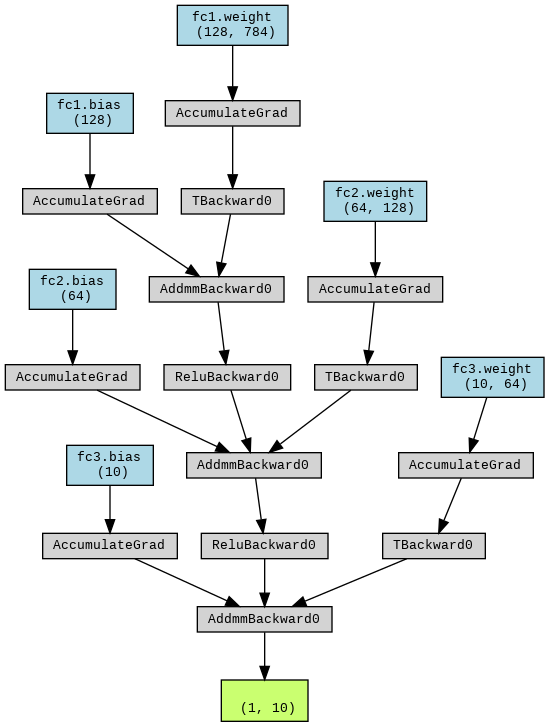
\includegraphics{superposition_files/figure-pdf/cell-6-output-1.png}

To keep things simple and accessible on a Colab with free resources (the
T4 GPU), we will use the canonical MNIST dataset of handwritten digits,
0-9.

Our training loop will run for five epochs and should complete within a
few minutes on the T4.

\begin{Shaded}
\begin{Highlighting}[]
\CommentTok{\# Load and preprocess the MNIST dataset}
\NormalTok{transform }\OperatorTok{=}\NormalTok{ transforms.Compose([transforms.ToTensor(), transforms.Normalize((}\FloatTok{0.1307}\NormalTok{,), (}\FloatTok{0.3081}\NormalTok{,))])}
\NormalTok{train\_dataset }\OperatorTok{=}\NormalTok{ datasets.MNIST(root}\OperatorTok{=}\StringTok{\textquotesingle{}./data\textquotesingle{}}\NormalTok{, train}\OperatorTok{=}\VariableTok{True}\NormalTok{, download}\OperatorTok{=}\VariableTok{True}\NormalTok{, transform}\OperatorTok{=}\NormalTok{transform)}
\NormalTok{train\_loader }\OperatorTok{=}\NormalTok{ torch.utils.data.DataLoader(train\_dataset, batch\_size}\OperatorTok{=}\DecValTok{64}\NormalTok{, shuffle}\OperatorTok{=}\VariableTok{True}\NormalTok{)}

\CommentTok{\# Define loss function and optimizer}
\NormalTok{criterion }\OperatorTok{=}\NormalTok{ nn.CrossEntropyLoss()}
\NormalTok{optimizer }\OperatorTok{=}\NormalTok{ optim.Adam(model.parameters())}

\CommentTok{\# Training loop}
\NormalTok{num\_epochs }\OperatorTok{=} \DecValTok{5}
\ControlFlowTok{for}\NormalTok{ epoch }\KeywordTok{in} \BuiltInTok{range}\NormalTok{(num\_epochs):  }\CommentTok{\# 5 epochs for demonstration}
    \ControlFlowTok{for}\NormalTok{ batch\_idx, (data, target) }\KeywordTok{in} \BuiltInTok{enumerate}\NormalTok{(train\_loader):}
\NormalTok{        data, target }\OperatorTok{=}\NormalTok{ data.to(device), target.to(device)}
\NormalTok{        optimizer.zero\_grad()}
\NormalTok{        output }\OperatorTok{=}\NormalTok{ model(data.view(data.size(}\DecValTok{0}\NormalTok{), }\OperatorTok{{-}}\DecValTok{1}\NormalTok{))}
\NormalTok{        loss }\OperatorTok{=}\NormalTok{ criterion(output, target)}
\NormalTok{        loss.backward()}
\NormalTok{        optimizer.step()}
    \ControlFlowTok{if}\NormalTok{ (epoch }\OperatorTok{+} \DecValTok{1}\NormalTok{) }\OperatorTok{\%} \DecValTok{1} \OperatorTok{==} \DecValTok{0}\NormalTok{:}
            \BuiltInTok{print}\NormalTok{(}\SpecialStringTok{f\textquotesingle{}Epoch [}\SpecialCharTok{\{}\NormalTok{epoch}\OperatorTok{+}\DecValTok{1}\SpecialCharTok{\}}\SpecialStringTok{/}\SpecialCharTok{\{}\NormalTok{num\_epochs}\SpecialCharTok{\}}\SpecialStringTok{], Loss: }\SpecialCharTok{\{}\NormalTok{loss}\SpecialCharTok{.}\NormalTok{item()}\SpecialCharTok{:.4f\}}\SpecialStringTok{\textquotesingle{}}\NormalTok{)}
\end{Highlighting}
\end{Shaded}

\begin{verbatim}
Epoch [1/5], Loss: 0.0020
Epoch [2/5], Loss: 0.0002
Epoch [3/5], Loss: 0.0047
Epoch [4/5], Loss: 0.0026
Epoch [5/5], Loss: 0.0004
\end{verbatim}

\subsection{Visualizing Weight
Matrices}\label{visualizing-weight-matrices}

One way to observe superposition is by visualizing the weight matrices
of our layers. We can plot these as heatmaps:

In these heatmaps, look for:

\begin{itemize}
\tightlist
\item
  Patterns or structure in the weights
\item
  Areas of high positive or negative values
\item
  Regions where weights seem to cancel each other out
\end{itemize}

Generally, we see the first layer has sparse weights. This is because it
connects directly to input pixels, many of which are not useful for
making predictions, for example, the white space. The network will learn
to assign very low weights to these less informative pixels.

In the second layer, we see a denser heatmap. Since this layer receives
input from the first layer's activations, these features are likely to
be meaningful and more evenly distributed for digit recognition. This
leads to a denser weight matrix, since the layer is using more of its
inputs.

\subsection{Relation to Superposition}\label{relation-to-superposition}

Even the sparsity in the first layer may hide some degree of
superposition, since the non-zero weights may be encoding multiple
features in a superimposed manner. This is especially likely since the
first layer ends up with fewer neurons than input dimensions.

Reminding ourselves of the architecture:

\begin{verbatim}
(fc1): Linear(in_features=784, out_features=128, bias=True)
\end{verbatim}

This means that the input features map to the 784 pixels of the MNIST
images inputs, however its \texttt{out\_features} reduces the
dimensionality to 128.

In the second layer, where low-level features are combined into more
abstract representations, superposition is noticeable as many patterns
are encoded efficiently in a limited number of neurons.

\begin{Shaded}
\begin{Highlighting}[]
\ImportTok{import}\NormalTok{ matplotlib.pyplot }\ImportTok{as}\NormalTok{ plt}
\ImportTok{import}\NormalTok{ seaborn }\ImportTok{as}\NormalTok{ sns}

\KeywordTok{def}\NormalTok{ plot\_weight\_matrix(weight\_matrix, title):}
\NormalTok{    plt.figure(figsize}\OperatorTok{=}\NormalTok{(}\DecValTok{8}\NormalTok{, }\DecValTok{6}\NormalTok{))}
\NormalTok{    sns.heatmap(weight\_matrix.cpu().detach().numpy(), cmap}\OperatorTok{=}\StringTok{\textquotesingle{}coolwarm\textquotesingle{}}\NormalTok{, center}\OperatorTok{=}\DecValTok{0}\NormalTok{)}
\NormalTok{    plt.title(title)}
\NormalTok{    plt.show()}

\NormalTok{plot\_weight\_matrix(model.fc1.weight, }\StringTok{"First Layer Weights"}\NormalTok{)}
\NormalTok{plot\_weight\_matrix(model.fc2.weight, }\StringTok{"Second Layer Weights"}\NormalTok{)}
\end{Highlighting}
\end{Shaded}

\includegraphics{superposition_files/figure-pdf/cell-8-output-1.png}

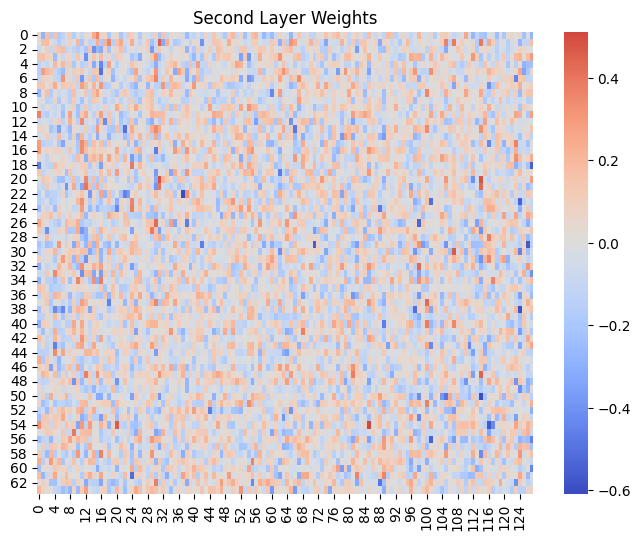
\includegraphics{superposition_files/figure-pdf/cell-8-output-2.png}

\subsection{Analyzing Activations}\label{analyzing-activations}

Another approach is to analyze the activations of neurons in response to
different inputs:

\begin{Shaded}
\begin{Highlighting}[]
\KeywordTok{def}\NormalTok{ get\_activations(model, input\_data):}
\NormalTok{    activations }\OperatorTok{=}\NormalTok{ \{\}}

    \KeywordTok{def}\NormalTok{ hook\_fn(module, }\BuiltInTok{input}\NormalTok{, output):}
\NormalTok{        activations[module] }\OperatorTok{=}\NormalTok{ output.detach()}

    \ControlFlowTok{for}\NormalTok{ name, module }\KeywordTok{in}\NormalTok{ model.named\_modules():}
        \ControlFlowTok{if} \BuiltInTok{isinstance}\NormalTok{(module, nn.Linear):}
\NormalTok{            module.register\_forward\_hook(hook\_fn)}
\NormalTok{    input\_data }\OperatorTok{=}\NormalTok{ input\_data.to(device)}
\NormalTok{    model(input\_data)}
    \ControlFlowTok{return}\NormalTok{ activations}

\CommentTok{\# Get a batch of test data}
\NormalTok{test\_loader }\OperatorTok{=}\NormalTok{ torch.utils.data.DataLoader(}
\NormalTok{    datasets.MNIST(root}\OperatorTok{=}\StringTok{\textquotesingle{}./data\textquotesingle{}}\NormalTok{, train}\OperatorTok{=}\VariableTok{False}\NormalTok{, transform}\OperatorTok{=}\NormalTok{transform),}
\NormalTok{    batch\_size}\OperatorTok{=}\DecValTok{64}\NormalTok{, shuffle}\OperatorTok{=}\VariableTok{True}\NormalTok{)}
\NormalTok{test\_data, \_ }\OperatorTok{=} \BuiltInTok{next}\NormalTok{(}\BuiltInTok{iter}\NormalTok{(test\_loader))}

\NormalTok{activations }\OperatorTok{=}\NormalTok{ get\_activations(model, test\_data.view(test\_data.size(}\DecValTok{0}\NormalTok{), }\OperatorTok{{-}}\DecValTok{1}\NormalTok{))}

\CommentTok{\# Plot activation distributions}
\ControlFlowTok{for}\NormalTok{ name, activation }\KeywordTok{in}\NormalTok{ activations.items():}
\NormalTok{    plt.figure(figsize}\OperatorTok{=}\NormalTok{(}\DecValTok{10}\NormalTok{, }\DecValTok{6}\NormalTok{))}
\NormalTok{    plt.hist(activation.cpu().numpy().flatten(), bins}\OperatorTok{=}\DecValTok{50}\NormalTok{)}
\NormalTok{    plt.title(}\SpecialStringTok{f"Activation Distribution for }\SpecialCharTok{\{}\NormalTok{name}\SpecialCharTok{\}}\SpecialStringTok{"}\NormalTok{)}
\NormalTok{    plt.xlabel(}\StringTok{"Activation Value"}\NormalTok{)}
\NormalTok{    plt.ylabel(}\StringTok{"Frequency"}\NormalTok{)}
\NormalTok{    plt.show()}
\end{Highlighting}
\end{Shaded}

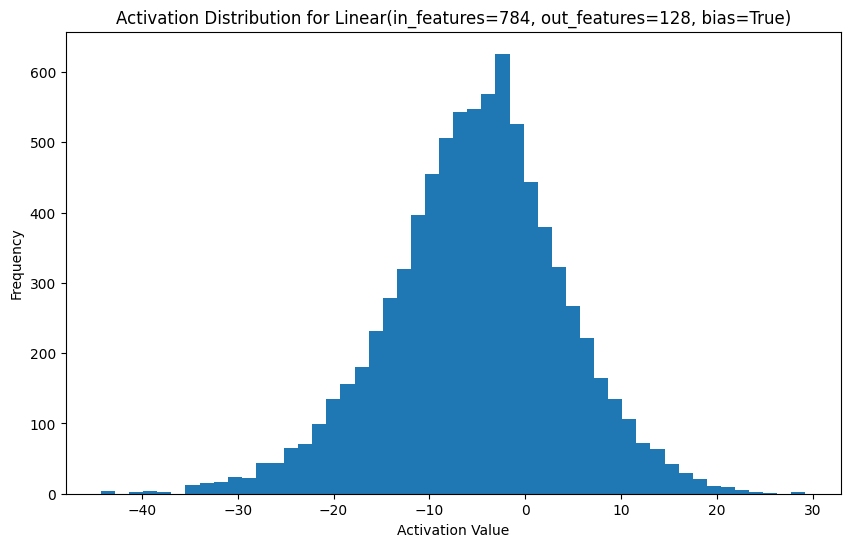
\includegraphics{superposition_files/figure-pdf/cell-9-output-1.png}

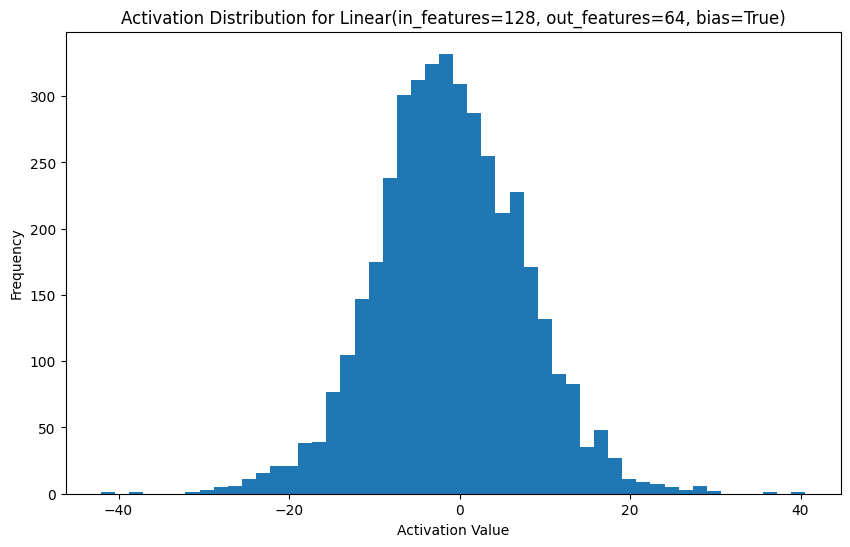
\includegraphics{superposition_files/figure-pdf/cell-9-output-2.png}

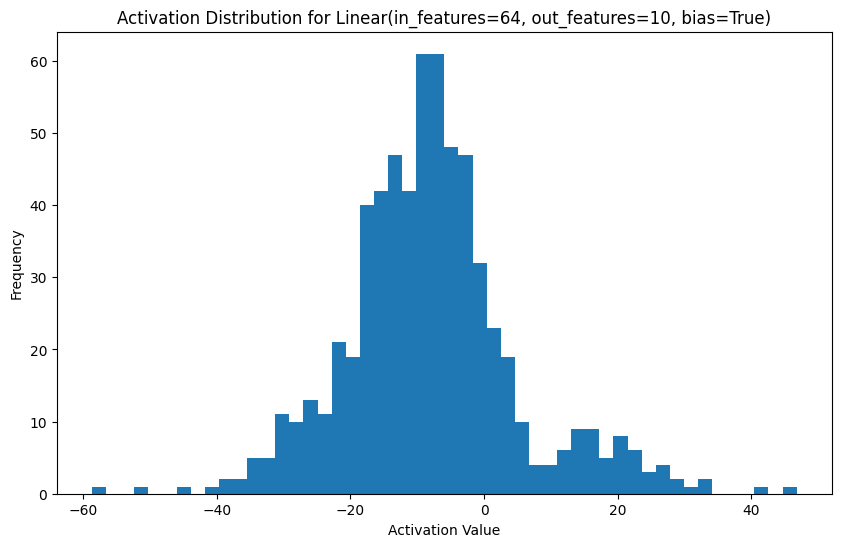
\includegraphics{superposition_files/figure-pdf/cell-9-output-3.png}

\subsection{Measuring Superposition}\label{measuring-superposition}

To quantify superposition, we can use techniques like Singular Value
Decomposition (SVD) on the weight matrices.

SVD is a technique in linear algebra to distill matrices into simpler
component matrices.

In this example, we take the following steps (also commented in the
code):

\begin{itemize}
\tightlist
\item
  Compute total variance, which is the sum of squared singular values
\item
  Calculate the cumulative variance of each singular value
\end{itemize}

\subsubsection{Interpretation}\label{interpretation}

The `effective rank' is a measure of superposition. A lower effective
rank indicated less of the phenonemon. A higher effective rank suggests
more, implying the weight matrix requires more dimensions to be
accurately represented.

\begin{Shaded}
\begin{Highlighting}[]
\ImportTok{import}\NormalTok{ numpy }\ImportTok{as}\NormalTok{ np}

\KeywordTok{def}\NormalTok{ analyze\_superposition(weight\_matrix):}
    \CommentTok{\# Here\textquotesingle{}s the SVD calculation. The \textquotesingle{}S\textquotesingle{} array contains the}
    \CommentTok{\# singular values in descending order.}
\NormalTok{    U, S, Vt }\OperatorTok{=}\NormalTok{ np.linalg.svd(weight\_matrix.cpu().detach().numpy())}

    \CommentTok{\# Plot singular values}
\NormalTok{    plt.figure(figsize}\OperatorTok{=}\NormalTok{(}\DecValTok{10}\NormalTok{, }\DecValTok{6}\NormalTok{))}
\NormalTok{    plt.plot(S)}
\NormalTok{    plt.title(}\StringTok{"Singular Values of Weight Matrix"}\NormalTok{)}
\NormalTok{    plt.xlabel(}\StringTok{"Index"}\NormalTok{)}
\NormalTok{    plt.ylabel(}\StringTok{"Singular Value"}\NormalTok{)}
\NormalTok{    plt.yscale(}\StringTok{\textquotesingle{}log\textquotesingle{}}\NormalTok{)}
\NormalTok{    plt.show()}

    \CommentTok{\# Calculate \textquotesingle{}effective rank\textquotesingle{}, which is a measure of superposition.}
    \CommentTok{\# This computes the total variance (sum of squared values), then}
    \CommentTok{\# calculates the cumulative variance explained by each singular value.}
\NormalTok{    total\_variance }\OperatorTok{=}\NormalTok{ np.}\BuiltInTok{sum}\NormalTok{(S}\OperatorTok{**}\DecValTok{2}\NormalTok{)}
\NormalTok{    cumulative\_variance }\OperatorTok{=}\NormalTok{ np.cumsum(S}\OperatorTok{**}\DecValTok{2}\NormalTok{) }\OperatorTok{/}\NormalTok{ total\_variance}
\NormalTok{    effective\_rank }\OperatorTok{=}\NormalTok{ np.}\BuiltInTok{sum}\NormalTok{(cumulative\_variance }\OperatorTok{\textless{}} \FloatTok{0.99}\NormalTok{)  }\CommentTok{\# 99\% of variance}

    \BuiltInTok{print}\NormalTok{(}\SpecialStringTok{f"Effective Rank: }\SpecialCharTok{\{}\NormalTok{effective\_rank}\SpecialCharTok{\}}\SpecialStringTok{"}\NormalTok{)}

\NormalTok{analyze\_superposition(model.fc1.weight)}
\NormalTok{analyze\_superposition(model.fc2.weight)}
\end{Highlighting}
\end{Shaded}

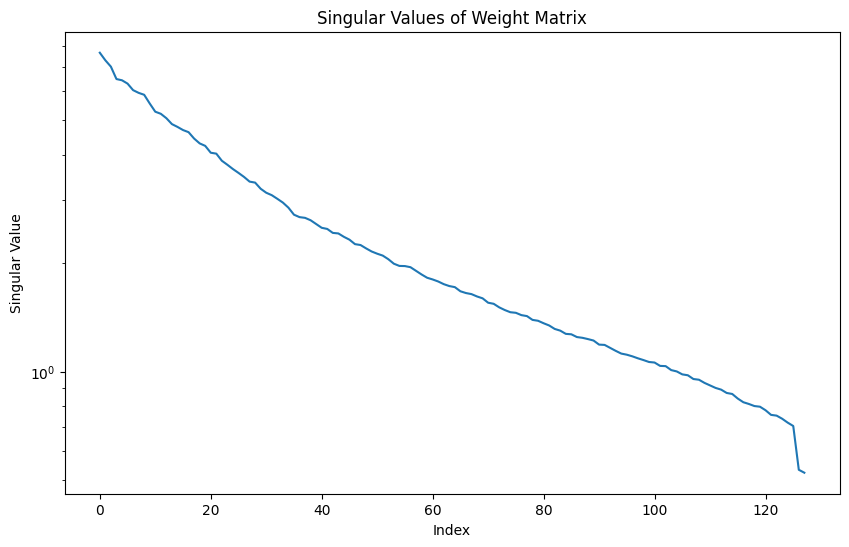
\includegraphics{superposition_files/figure-pdf/cell-10-output-1.png}

\begin{verbatim}
Effective Rank: 110
\end{verbatim}

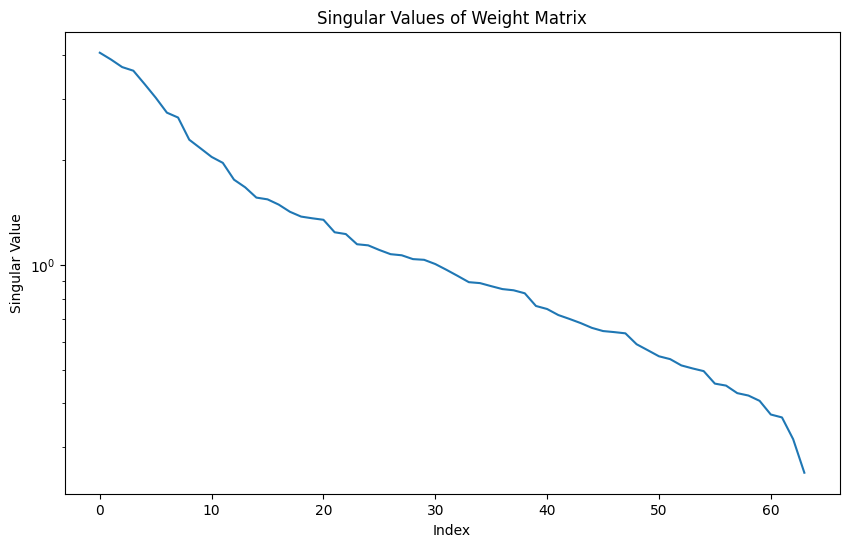
\includegraphics{superposition_files/figure-pdf/cell-10-output-3.png}

\begin{verbatim}
Effective Rank: 54
\end{verbatim}

In our SimpleNet model, we defined the following architecture:

\begin{Shaded}
\begin{Highlighting}[]

\KeywordTok{class}\NormalTok{ SimpleNet(nn.Module):}
    \KeywordTok{def} \FunctionTok{\_\_init\_\_}\NormalTok{(}\VariableTok{self}\NormalTok{):}
        \BuiltInTok{super}\NormalTok{(SimpleNet, }\VariableTok{self}\NormalTok{).}\FunctionTok{\_\_init\_\_}\NormalTok{()}
        \VariableTok{self}\NormalTok{.fc1 }\OperatorTok{=}\NormalTok{ nn.Linear(}\DecValTok{784}\NormalTok{, }\DecValTok{128}\NormalTok{)}
        \VariableTok{self}\NormalTok{.fc2 }\OperatorTok{=}\NormalTok{ nn.Linear(}\DecValTok{128}\NormalTok{, }\DecValTok{64}\NormalTok{)}
        \VariableTok{self}\NormalTok{.fc3 }\OperatorTok{=}\NormalTok{ nn.Linear(}\DecValTok{64}\NormalTok{, }\DecValTok{10}\NormalTok{)}
\end{Highlighting}
\end{Shaded}

Let's compare the effective ranks we observed with the actual number of
neurons in each layer:

First layer (fc1):

Total neurons: 128 Effective rank: 113 Ratio: 113 / 128 ≈ 0.883 or
88.3\%

Second layer (fc2):

Total neurons: 64 Effective rank: 54 Ratio: 54 / 64 ≈ 0.844 or 84.4\%

Interpretation:

First layer (fc1): The effective rank of 113 compared to 128 total
neurons suggests that this layer is using about 88.3\% of its capacity
for unique features, corresponding to a high degree of superposition. So
a large number of singular values are needed to explain the variance in
the weight matricies.

Second layer (fc2): The effective rank of 54 vs 64 total neurons
indicates that this layer is using about 84.4\% of its capacity for
unique features, showing a slight decrease that may indicate more
specialization or feature abstraction in the second layer.

The effective rank gives us an idea of how many ``effective features''
the layer is representing. A higher effective rank compared to the
actual number of neurons suggests neurons are representing multiple
features simultaneously, indicating a higher degree of superposition.

\subsection{Interpreting the Results}\label{interpreting-the-results}

When looking at the results, focus on sparse activation patterns, which
might indicate specialized neurons. Compare the number of neurons to the
effective rank - a large discrepancy suggests a high degree of
superposition. Observe how superposition changes across layers. Consider
how different input patterns affect the activations and whether this
reveals any superposed features.

\subsection{More layers, more data: CIFAR
100}\label{more-layers-more-data-cifar-100}

Let's explore whether larger datasets and more complex neural network
architectures affect the degree of superposition.

We switch to the ResNet50 model, which has 50 layers, including 48
convolutional layers, 1 max pool and 1 average pool layer. It uses skip
connections to address the vanishing gradient problem, enabling training
of deeper networks.

We will use the CIFAR-100 dataset, which comprises 60,000, 32 x 32 color
images in 100 classes.

\begin{Shaded}
\begin{Highlighting}[]
\ImportTok{import}\NormalTok{ torch}
\ImportTok{import}\NormalTok{ torch.nn }\ImportTok{as}\NormalTok{ nn}
\ImportTok{import}\NormalTok{ torch.optim }\ImportTok{as}\NormalTok{ optim}
\ImportTok{from}\NormalTok{ torchvision }\ImportTok{import}\NormalTok{ models, datasets, transforms}
\ImportTok{from}\NormalTok{ torch.utils.data }\ImportTok{import}\NormalTok{ DataLoader}
\ImportTok{import}\NormalTok{ matplotlib.pyplot }\ImportTok{as}\NormalTok{ plt}
\ImportTok{import}\NormalTok{ seaborn }\ImportTok{as}\NormalTok{ sns}
\ImportTok{import}\NormalTok{ numpy }\ImportTok{as}\NormalTok{ np}
\ImportTok{from}\NormalTok{ tqdm }\ImportTok{import}\NormalTok{ tqdm}

\CommentTok{\# Check if CUDA is available}
\NormalTok{device }\OperatorTok{=}\NormalTok{ torch.device(}\StringTok{"cuda"} \ControlFlowTok{if}\NormalTok{ torch.cuda.is\_available() }\ControlFlowTok{else} \StringTok{"cpu"}\NormalTok{)}
\BuiltInTok{print}\NormalTok{(}\SpecialStringTok{f"Using device: }\SpecialCharTok{\{}\NormalTok{device}\SpecialCharTok{\}}\SpecialStringTok{"}\NormalTok{)}

\CommentTok{\# Define transforms}
\NormalTok{transform\_train }\OperatorTok{=}\NormalTok{ transforms.Compose([}
\NormalTok{    transforms.RandomCrop(}\DecValTok{32}\NormalTok{, padding}\OperatorTok{=}\DecValTok{4}\NormalTok{),}
\NormalTok{    transforms.RandomHorizontalFlip(),}
\NormalTok{    transforms.ToTensor(),}
\NormalTok{    transforms.Normalize((}\FloatTok{0.5071}\NormalTok{, }\FloatTok{0.4867}\NormalTok{, }\FloatTok{0.4408}\NormalTok{), (}\FloatTok{0.2675}\NormalTok{, }\FloatTok{0.2565}\NormalTok{, }\FloatTok{0.2761}\NormalTok{)),}
\NormalTok{])}

\NormalTok{transform\_test }\OperatorTok{=}\NormalTok{ transforms.Compose([}
\NormalTok{    transforms.ToTensor(),}
\NormalTok{    transforms.Normalize((}\FloatTok{0.5071}\NormalTok{, }\FloatTok{0.4867}\NormalTok{, }\FloatTok{0.4408}\NormalTok{), (}\FloatTok{0.2675}\NormalTok{, }\FloatTok{0.2565}\NormalTok{, }\FloatTok{0.2761}\NormalTok{)),}
\NormalTok{])}

\CommentTok{\# Load CIFAR{-}100 dataset}
\NormalTok{train\_dataset }\OperatorTok{=}\NormalTok{ datasets.CIFAR100(root}\OperatorTok{=}\StringTok{\textquotesingle{}./data\textquotesingle{}}\NormalTok{, train}\OperatorTok{=}\VariableTok{True}\NormalTok{, download}\OperatorTok{=}\VariableTok{True}\NormalTok{, transform}\OperatorTok{=}\NormalTok{transform\_train)}
\NormalTok{test\_dataset }\OperatorTok{=}\NormalTok{ datasets.CIFAR100(root}\OperatorTok{=}\StringTok{\textquotesingle{}./data\textquotesingle{}}\NormalTok{, train}\OperatorTok{=}\VariableTok{False}\NormalTok{, download}\OperatorTok{=}\VariableTok{True}\NormalTok{, transform}\OperatorTok{=}\NormalTok{transform\_test)}

\CommentTok{\# Create data loaders}
\NormalTok{train\_loader }\OperatorTok{=}\NormalTok{ DataLoader(train\_dataset, batch\_size}\OperatorTok{=}\DecValTok{128}\NormalTok{, shuffle}\OperatorTok{=}\VariableTok{True}\NormalTok{, num\_workers}\OperatorTok{=}\DecValTok{4}\NormalTok{, pin\_memory}\OperatorTok{=}\VariableTok{True}\NormalTok{)}
\NormalTok{test\_loader }\OperatorTok{=}\NormalTok{ DataLoader(test\_dataset, batch\_size}\OperatorTok{=}\DecValTok{128}\NormalTok{, shuffle}\OperatorTok{=}\VariableTok{False}\NormalTok{, num\_workers}\OperatorTok{=}\DecValTok{4}\NormalTok{, pin\_memory}\OperatorTok{=}\VariableTok{True}\NormalTok{)}

\CommentTok{\# Load pre{-}trained ResNet50 model and modify for CIFAR{-}100}
\NormalTok{model }\OperatorTok{=}\NormalTok{ models.resnet50(pretrained}\OperatorTok{=}\VariableTok{True}\NormalTok{)}
\NormalTok{model.fc }\OperatorTok{=}\NormalTok{ nn.Linear(model.fc.in\_features, }\DecValTok{100}\NormalTok{)  }\CommentTok{\# 100 classes in CIFAR{-}100}
\NormalTok{model }\OperatorTok{=}\NormalTok{ model.to(device)}

\CommentTok{\# Define loss function and optimizer}
\NormalTok{criterion }\OperatorTok{=}\NormalTok{ nn.CrossEntropyLoss()}
\NormalTok{optimizer }\OperatorTok{=}\NormalTok{ optim.Adam(model.parameters(), lr}\OperatorTok{=}\FloatTok{0.001}\NormalTok{)}

\CommentTok{\# Training loop}
\NormalTok{num\_epochs }\OperatorTok{=} \DecValTok{10}
\ControlFlowTok{for}\NormalTok{ epoch }\KeywordTok{in} \BuiltInTok{range}\NormalTok{(num\_epochs):}
\NormalTok{    model.train()}
\NormalTok{    running\_loss }\OperatorTok{=} \FloatTok{0.0}
    \ControlFlowTok{for}\NormalTok{ inputs, labels }\KeywordTok{in}\NormalTok{ tqdm(train\_loader, desc}\OperatorTok{=}\SpecialStringTok{f"Epoch }\SpecialCharTok{\{}\NormalTok{epoch}\OperatorTok{+}\DecValTok{1}\SpecialCharTok{\}}\SpecialStringTok{/}\SpecialCharTok{\{}\NormalTok{num\_epochs}\SpecialCharTok{\}}\SpecialStringTok{"}\NormalTok{):}
\NormalTok{        inputs, labels }\OperatorTok{=}\NormalTok{ inputs.to(device), labels.to(device)}

\NormalTok{        optimizer.zero\_grad()}
\NormalTok{        outputs }\OperatorTok{=}\NormalTok{ model(inputs)}
\NormalTok{        loss }\OperatorTok{=}\NormalTok{ criterion(outputs, labels)}
\NormalTok{        loss.backward()}
\NormalTok{        optimizer.step()}

\NormalTok{        running\_loss }\OperatorTok{+=}\NormalTok{ loss.item()}

    \BuiltInTok{print}\NormalTok{(}\SpecialStringTok{f"Epoch }\SpecialCharTok{\{}\NormalTok{epoch}\OperatorTok{+}\DecValTok{1}\SpecialCharTok{\}}\SpecialStringTok{ loss: }\SpecialCharTok{\{}\NormalTok{running\_loss}\OperatorTok{/}\BuiltInTok{len}\NormalTok{(train\_loader)}\SpecialCharTok{:.4f\}}\SpecialStringTok{"}\NormalTok{)}

    \CommentTok{\# Validation}
\NormalTok{    model.}\BuiltInTok{eval}\NormalTok{()}
\NormalTok{    correct }\OperatorTok{=} \DecValTok{0}
\NormalTok{    total }\OperatorTok{=} \DecValTok{0}
    \ControlFlowTok{with}\NormalTok{ torch.no\_grad():}
        \ControlFlowTok{for}\NormalTok{ inputs, labels }\KeywordTok{in}\NormalTok{ tqdm(test\_loader, desc}\OperatorTok{=}\StringTok{"Validation"}\NormalTok{):}
\NormalTok{            inputs, labels }\OperatorTok{=}\NormalTok{ inputs.to(device), labels.to(device)}
\NormalTok{            outputs }\OperatorTok{=}\NormalTok{ model(inputs)}
\NormalTok{            \_, predicted }\OperatorTok{=}\NormalTok{ outputs.}\BuiltInTok{max}\NormalTok{(}\DecValTok{1}\NormalTok{)}
\NormalTok{            total }\OperatorTok{+=}\NormalTok{ labels.size(}\DecValTok{0}\NormalTok{)}
\NormalTok{            correct }\OperatorTok{+=}\NormalTok{ predicted.eq(labels).}\BuiltInTok{sum}\NormalTok{().item()}

    \BuiltInTok{print}\NormalTok{(}\SpecialStringTok{f"Validation Accuracy: }\SpecialCharTok{\{}\FloatTok{100.}\OperatorTok{*}\NormalTok{correct}\OperatorTok{/}\NormalTok{total}\SpecialCharTok{:.2f\}}\SpecialStringTok{\%"}\NormalTok{)}

\BuiltInTok{print}\NormalTok{(}\StringTok{"Training completed"}\NormalTok{)}

\end{Highlighting}
\end{Shaded}

\begin{verbatim}
Using device: cuda
Downloading https://www.cs.toronto.edu/~kriz/cifar-100-python.tar.gz to ./data/cifar-100-python.tar.gz
\end{verbatim}

\begin{verbatim}
100%|██████████| 169001437/169001437 [00:04<00:00, 42237449.26it/s]
\end{verbatim}

\begin{verbatim}
Extracting ./data/cifar-100-python.tar.gz to ./data
Files already downloaded and verified
\end{verbatim}

\begin{verbatim}
/usr/local/lib/python3.10/dist-packages/torch/utils/data/dataloader.py:557: UserWarning: This DataLoader will create 4 worker processes in total. Our suggested max number of worker in current system is 2, which is smaller than what this DataLoader is going to create. Please be aware that excessive worker creation might get DataLoader running slow or even freeze, lower the worker number to avoid potential slowness/freeze if necessary.
  warnings.warn(_create_warning_msg(
/usr/local/lib/python3.10/dist-packages/torchvision/models/_utils.py:208: UserWarning: The parameter 'pretrained' is deprecated since 0.13 and may be removed in the future, please use 'weights' instead.
  warnings.warn(
/usr/local/lib/python3.10/dist-packages/torchvision/models/_utils.py:223: UserWarning: Arguments other than a weight enum or `None` for 'weights' are deprecated since 0.13 and may be removed in the future. The current behavior is equivalent to passing `weights=ResNet50_Weights.IMAGENET1K_V1`. You can also use `weights=ResNet50_Weights.DEFAULT` to get the most up-to-date weights.
  warnings.warn(msg)
Downloading: "https://download.pytorch.org/models/resnet50-0676ba61.pth" to /root/.cache/torch/hub/checkpoints/resnet50-0676ba61.pth
100%|██████████| 97.8M/97.8M [00:00<00:00, 130MB/s]
Epoch 1/10: 100%|██████████| 391/391 [00:34<00:00, 11.18it/s]
\end{verbatim}

\begin{verbatim}
Epoch 1 loss: 3.3070
\end{verbatim}

\begin{verbatim}
Validation: 100%|██████████| 79/79 [00:03<00:00, 24.33it/s]
\end{verbatim}

\begin{verbatim}
Validation Accuracy: 25.89%
\end{verbatim}

\begin{verbatim}
Epoch 2/10: 100%|██████████| 391/391 [00:33<00:00, 11.58it/s]
\end{verbatim}

\begin{verbatim}
Epoch 2 loss: 2.5782
\end{verbatim}

\begin{verbatim}
Validation: 100%|██████████| 79/79 [00:03<00:00, 19.93it/s]
\end{verbatim}

\begin{verbatim}
Validation Accuracy: 41.69%
\end{verbatim}

\begin{verbatim}
Epoch 3/10: 100%|██████████| 391/391 [00:34<00:00, 11.28it/s]
\end{verbatim}

\begin{verbatim}
Epoch 3 loss: 2.1787
\end{verbatim}

\begin{verbatim}
Validation: 100%|██████████| 79/79 [00:03<00:00, 23.63it/s]
\end{verbatim}

\begin{verbatim}
Validation Accuracy: 45.72%
\end{verbatim}

\begin{verbatim}
Epoch 4/10: 100%|██████████| 391/391 [00:33<00:00, 11.62it/s]
\end{verbatim}

\begin{verbatim}
Epoch 4 loss: 2.0079
\end{verbatim}

\begin{verbatim}
Validation: 100%|██████████| 79/79 [00:03<00:00, 25.49it/s]
\end{verbatim}

\begin{verbatim}
Validation Accuracy: 48.87%
\end{verbatim}

\begin{verbatim}
Epoch 5/10: 100%|██████████| 391/391 [00:33<00:00, 11.72it/s]
\end{verbatim}

\begin{verbatim}
Epoch 5 loss: 1.7884
\end{verbatim}

\begin{verbatim}
Validation: 100%|██████████| 79/79 [00:05<00:00, 15.58it/s]
\end{verbatim}

\begin{verbatim}
Validation Accuracy: 50.87%
\end{verbatim}

\begin{verbatim}
Epoch 6/10: 100%|██████████| 391/391 [00:33<00:00, 11.65it/s]
\end{verbatim}

\begin{verbatim}
Epoch 6 loss: 1.6728
\end{verbatim}

\begin{verbatim}
Validation: 100%|██████████| 79/79 [00:03<00:00, 25.56it/s]
\end{verbatim}

\begin{verbatim}
Validation Accuracy: 51.85%
\end{verbatim}

\begin{verbatim}
Epoch 7/10: 100%|██████████| 391/391 [00:33<00:00, 11.60it/s]
\end{verbatim}

\begin{verbatim}
Epoch 7 loss: 1.5569
\end{verbatim}

\begin{verbatim}
Validation: 100%|██████████| 79/79 [00:03<00:00, 25.69it/s]
\end{verbatim}

\begin{verbatim}
Validation Accuracy: 53.72%
\end{verbatim}

\begin{verbatim}
Epoch 8/10: 100%|██████████| 391/391 [00:34<00:00, 11.41it/s]
\end{verbatim}

\begin{verbatim}
Epoch 8 loss: 1.4626
\end{verbatim}

\begin{verbatim}
Validation: 100%|██████████| 79/79 [00:04<00:00, 15.99it/s]
\end{verbatim}

\begin{verbatim}
Validation Accuracy: 53.80%
\end{verbatim}

\begin{verbatim}
Epoch 9/10: 100%|██████████| 391/391 [00:34<00:00, 11.32it/s]
\end{verbatim}

\begin{verbatim}
Epoch 9 loss: 1.4110
\end{verbatim}

\begin{verbatim}
Validation: 100%|██████████| 79/79 [00:03<00:00, 24.77it/s]
\end{verbatim}

\begin{verbatim}
Validation Accuracy: 54.18%
\end{verbatim}

\begin{verbatim}
Epoch 10/10: 100%|██████████| 391/391 [00:33<00:00, 11.73it/s]
\end{verbatim}

\begin{verbatim}
Epoch 10 loss: 1.3250
\end{verbatim}

\begin{verbatim}
Validation: 100%|██████████| 79/79 [00:03<00:00, 24.64it/s]
\end{verbatim}

\begin{verbatim}
Validation Accuracy: 55.82%
Training completed
\end{verbatim}

\begin{verbatim}
\end{verbatim}

\begin{Shaded}
\begin{Highlighting}[]
\ImportTok{import}\NormalTok{ pandas }\ImportTok{as}\NormalTok{ pd}
\ImportTok{import}\NormalTok{ matplotlib.pyplot }\ImportTok{as}\NormalTok{ plt}
\ImportTok{import}\NormalTok{ seaborn }\ImportTok{as}\NormalTok{ sns}
\ImportTok{from}\NormalTok{ collections }\ImportTok{import}\NormalTok{ OrderedDict}

\KeywordTok{def}\NormalTok{ get\_activations(model, loader, num\_batches}\OperatorTok{=}\DecValTok{10}\NormalTok{):}
\NormalTok{    activations }\OperatorTok{=}\NormalTok{ OrderedDict()}

    \KeywordTok{def}\NormalTok{ hook\_fn(name):}
        \KeywordTok{def}\NormalTok{ hook(module, }\BuiltInTok{input}\NormalTok{, output):}
\NormalTok{            activations[name] }\OperatorTok{=}\NormalTok{ output.cpu().detach()}
        \ControlFlowTok{return}\NormalTok{ hook}

    \CommentTok{\# Register hooks for convolutional layers}
    \ControlFlowTok{for}\NormalTok{ name, module }\KeywordTok{in}\NormalTok{ model.named\_modules():}
        \ControlFlowTok{if} \BuiltInTok{isinstance}\NormalTok{(module, nn.Conv2d):}
\NormalTok{            module.register\_forward\_hook(hook\_fn(name))}

\NormalTok{    model.}\BuiltInTok{eval}\NormalTok{()}
    \ControlFlowTok{with}\NormalTok{ torch.no\_grad():}
        \ControlFlowTok{for}\NormalTok{ i, (inputs, \_) }\KeywordTok{in} \BuiltInTok{enumerate}\NormalTok{(loader):}
            \ControlFlowTok{if}\NormalTok{ i }\OperatorTok{\textgreater{}=}\NormalTok{ num\_batches:}
                \ControlFlowTok{break}
\NormalTok{            inputs }\OperatorTok{=}\NormalTok{ inputs.to(device)}
\NormalTok{            \_ }\OperatorTok{=}\NormalTok{ model(inputs)}

    \ControlFlowTok{return}\NormalTok{ activations}

\KeywordTok{def}\NormalTok{ analyze\_superposition(activation, layer\_name):}
\NormalTok{    reshaped }\OperatorTok{=}\NormalTok{ activation.reshape(activation.shape[}\DecValTok{1}\NormalTok{], }\OperatorTok{{-}}\DecValTok{1}\NormalTok{).numpy()}
\NormalTok{    U, S, Vt }\OperatorTok{=}\NormalTok{ np.linalg.svd(reshaped, full\_matrices}\OperatorTok{=}\VariableTok{False}\NormalTok{)}

\NormalTok{    total\_variance }\OperatorTok{=}\NormalTok{ np.}\BuiltInTok{sum}\NormalTok{(S}\OperatorTok{**}\DecValTok{2}\NormalTok{)}
\NormalTok{    cumulative\_variance }\OperatorTok{=}\NormalTok{ np.cumsum(S}\OperatorTok{**}\DecValTok{2}\NormalTok{) }\OperatorTok{/}\NormalTok{ total\_variance}
\NormalTok{    effective\_rank }\OperatorTok{=}\NormalTok{ np.}\BuiltInTok{sum}\NormalTok{(cumulative\_variance }\OperatorTok{\textless{}} \FloatTok{0.99}\NormalTok{)  }\CommentTok{\# 99\% of variance}

    \ControlFlowTok{return}\NormalTok{ \{}
        \StringTok{\textquotesingle{}layer\_name\textquotesingle{}}\NormalTok{: layer\_name,}
        \StringTok{\textquotesingle{}total\_channels\textquotesingle{}}\NormalTok{: activation.shape[}\DecValTok{1}\NormalTok{],}
        \StringTok{\textquotesingle{}effective\_rank\textquotesingle{}}\NormalTok{: effective\_rank,}
        \StringTok{\textquotesingle{}ratio\textquotesingle{}}\NormalTok{: effective\_rank }\OperatorTok{/}\NormalTok{ activation.shape[}\DecValTok{1}\NormalTok{]}
\NormalTok{    \}}

\CommentTok{\# Get activations}
\NormalTok{activations }\OperatorTok{=}\NormalTok{ get\_activations(model, test\_loader)}

\CommentTok{\# Analyze superposition for each layer}
\NormalTok{results }\OperatorTok{=}\NormalTok{ []}
\ControlFlowTok{for}\NormalTok{ name, activation }\KeywordTok{in}\NormalTok{ activations.items():}
\NormalTok{    results.append(analyze\_superposition(activation, name))}

\CommentTok{\# Create DataFrame}
\NormalTok{df }\OperatorTok{=}\NormalTok{ pd.DataFrame(results)}

\CommentTok{\# Plot effective rank vs layer}
\NormalTok{plt.figure(figsize}\OperatorTok{=}\NormalTok{(}\DecValTok{12}\NormalTok{, }\DecValTok{6}\NormalTok{))}
\NormalTok{sns.lineplot(data}\OperatorTok{=}\NormalTok{df, x}\OperatorTok{=}\NormalTok{df.index, y}\OperatorTok{=}\StringTok{\textquotesingle{}effective\_rank\textquotesingle{}}\NormalTok{, marker}\OperatorTok{=}\StringTok{\textquotesingle{}o\textquotesingle{}}\NormalTok{)}
\NormalTok{plt.title(}\StringTok{\textquotesingle{}Effective Rank vs Layer\textquotesingle{}}\NormalTok{)}
\NormalTok{plt.xlabel(}\StringTok{\textquotesingle{}Layer Index\textquotesingle{}}\NormalTok{)}
\NormalTok{plt.ylabel(}\StringTok{\textquotesingle{}Effective Rank\textquotesingle{}}\NormalTok{)}
\NormalTok{plt.xticks(df.index, df[}\StringTok{\textquotesingle{}layer\_name\textquotesingle{}}\NormalTok{], rotation}\OperatorTok{=}\DecValTok{45}\NormalTok{, ha}\OperatorTok{=}\StringTok{\textquotesingle{}right\textquotesingle{}}\NormalTok{)}
\NormalTok{plt.tight\_layout()}
\NormalTok{plt.savefig(}\StringTok{\textquotesingle{}effective\_rank\_vs\_layer.png\textquotesingle{}}\NormalTok{)}
\NormalTok{plt.close()}

\CommentTok{\# Plot ratio of effective rank to total channels}
\NormalTok{plt.figure(figsize}\OperatorTok{=}\NormalTok{(}\DecValTok{12}\NormalTok{, }\DecValTok{6}\NormalTok{))}
\NormalTok{sns.lineplot(data}\OperatorTok{=}\NormalTok{df, x}\OperatorTok{=}\NormalTok{df.index, y}\OperatorTok{=}\StringTok{\textquotesingle{}ratio\textquotesingle{}}\NormalTok{, marker}\OperatorTok{=}\StringTok{\textquotesingle{}o\textquotesingle{}}\NormalTok{)}
\NormalTok{plt.title(}\StringTok{\textquotesingle{}Ratio of Effective Rank to Total Channels vs Layer\textquotesingle{}}\NormalTok{)}
\NormalTok{plt.xlabel(}\StringTok{\textquotesingle{}Layer Index\textquotesingle{}}\NormalTok{)}
\NormalTok{plt.ylabel(}\StringTok{\textquotesingle{}Ratio\textquotesingle{}}\NormalTok{)}
\NormalTok{plt.xticks(df.index, df[}\StringTok{\textquotesingle{}layer\_name\textquotesingle{}}\NormalTok{], rotation}\OperatorTok{=}\DecValTok{45}\NormalTok{, ha}\OperatorTok{=}\StringTok{\textquotesingle{}right\textquotesingle{}}\NormalTok{)}
\NormalTok{plt.tight\_layout()}
\NormalTok{plt.savefig(}\StringTok{\textquotesingle{}effective\_rank\_ratio\_vs\_layer.png\textquotesingle{}}\NormalTok{)}
\NormalTok{plt.close()}

\BuiltInTok{print}\NormalTok{(df)}
\BuiltInTok{print}\NormalTok{(}\StringTok{"}\CharTok{\textbackslash{}n}\StringTok{Analysis completed. Check the generated PNG files for visualizations."}\NormalTok{)}
\end{Highlighting}
\end{Shaded}

\begin{verbatim}
               layer_name  total_channels  effective_rank     ratio
0                   conv1              64              59  0.921875
1          layer1.0.conv1              64              49  0.765625
2          layer1.0.conv2              64              53  0.828125
3          layer1.0.conv3             256             139  0.542969
4   layer1.0.downsample.0             256             133  0.519531
5          layer1.1.conv1              64              59  0.921875
6          layer1.1.conv2              64              58  0.906250
7          layer1.1.conv3             256             202  0.789062
8          layer1.2.conv1              64              60  0.937500
9          layer1.2.conv2              64              60  0.937500
10         layer1.2.conv3             256             231  0.902344
11         layer2.0.conv1             128             112  0.875000
12         layer2.0.conv2             128             113  0.882812
13         layer2.0.conv3             512             419  0.818359
14  layer2.0.downsample.0             512             398  0.777344
15         layer2.1.conv1             128              99  0.773438
16         layer2.1.conv2             128              52  0.406250
17         layer2.1.conv3             512             229  0.447266
18         layer2.2.conv1             128             108  0.843750
19         layer2.2.conv2             128              87  0.679688
20         layer2.2.conv3             512             360  0.703125
21         layer2.3.conv1             128             110  0.859375
22         layer2.3.conv2             128              86  0.671875
23         layer2.3.conv3             512             372  0.726562
24         layer3.0.conv1             256             220  0.859375
25         layer3.0.conv2             256             169  0.660156
26         layer3.0.conv3            1024             344  0.335938
27  layer3.0.downsample.0            1024             385  0.375977
28         layer3.1.conv1             256             117  0.457031
29         layer3.1.conv2             256              50  0.195312
30         layer3.1.conv3            1024              78  0.076172
31         layer3.2.conv1             256             121  0.472656
32         layer3.2.conv2             256              44  0.171875
33         layer3.2.conv3            1024              83  0.081055
34         layer3.3.conv1             256             126  0.492188
35         layer3.3.conv2             256              41  0.160156
36         layer3.3.conv3            1024              25  0.024414
37         layer3.4.conv1             256             116  0.453125
38         layer3.4.conv2             256              26  0.101562
39         layer3.4.conv3            1024              25  0.024414
40         layer3.5.conv1             256             116  0.453125
41         layer3.5.conv2             256              32  0.125000
42         layer3.5.conv3            1024              29  0.028320
43         layer4.0.conv1             512             235  0.458984
44         layer4.0.conv2             512             100  0.195312
45         layer4.0.conv3            2048             121  0.059082
46  layer4.0.downsample.0            2048             116  0.056641
47         layer4.1.conv1             512              70  0.136719
48         layer4.1.conv2             512              46  0.089844
49         layer4.1.conv3            2048              43  0.020996
50         layer4.2.conv1             512              62  0.121094
51         layer4.2.conv2             512              58  0.113281
52         layer4.2.conv3            2048              27  0.013184

Analysis completed. Check the generated PNG files for visualizations.
\end{verbatim}

\subsection{Interpretation}\label{interpretation-1}

With some consistency, we see effective rank ratio decrease as the later
network layers learn more abstract representations.

\begin{Shaded}
\begin{Highlighting}[]
\CommentTok{\# Display the image in the notebook}
\NormalTok{image\_path }\OperatorTok{=} \StringTok{"/content/effective\_rank\_ratio\_vs\_layer.png"}
\NormalTok{display(Image(filename}\OperatorTok{=}\NormalTok{image\_path))}
\end{Highlighting}
\end{Shaded}

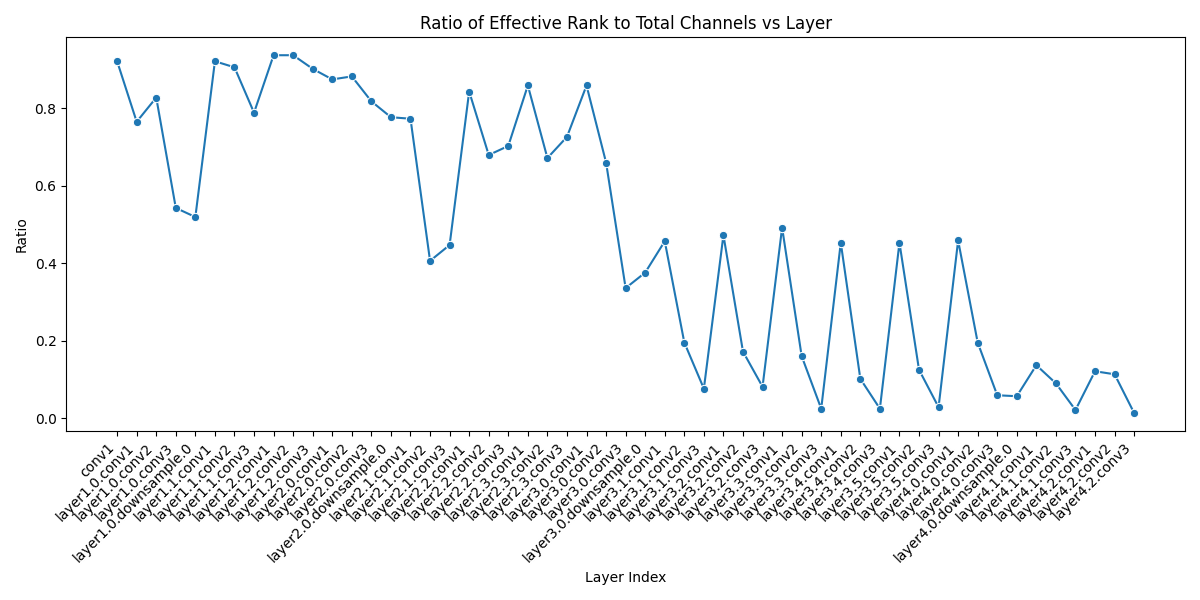
\includegraphics{superposition_files/figure-pdf/cell-13-output-1.png}

\bookmarksetup{startatroot}

\chapter{Interpreting Superposition Analysis
Results}\label{interpreting-superposition-analysis-results}

Let's analyze a result for one single convolutional layer

\begin{verbatim}
Conv2d(2048, 512, kernel_size=(1, 1), stride=(1, 1), bias=False):
Total channels: 512
Effective Rank: 67
Ratio: 0.13
\end{verbatim}

\begin{enumerate}
\def\labelenumi{\arabic{enumi}.}
\tightlist
\item
  Layer description:
  \texttt{Conv2d(2048,\ 512,\ kernel\_size=(1,\ 1),\ stride=(1,\ 1),\ bias=False)}

  \begin{itemize}
  \tightlist
  \item
    This is a 2D convolutional layer
  \item
    It takes 2048 input channels and outputs 512 channels
  \item
    It uses a 1x1 kernel size, which is essentially a pointwise
    convolution
  \end{itemize}
\item
  Total channels: 512

  \begin{itemize}
  \tightlist
  \item
    In a convolutional neural network, each channel can be thought of as
    a ``neuron'' or a feature detector
  \item
    So this layer has 512 ``neurons'' or feature detectors
  \end{itemize}
\item
  Effective Rank: 67

  \begin{itemize}
  \tightlist
  \item
    This is significantly lower than the number of channels (512),
    indicating a small subset of the available dimensions are needed to
    explain most of the variance in the weight matrix. This suggests low
    superposition, since the majority of channels are not contributing
    to complex representations.
  \end{itemize}
\item
  Ratio: 0.13 (67 / 512)

  \begin{itemize}
  \tightlist
  \item
    This ratio indicates that only about 13\% of the available
    dimensions are being effectively utilized
  \end{itemize}
\end{enumerate}

In summary, this result shows a lower degree of superposition, with the
layer using only about 67 effective dimensions to represent information,
despite having 512 channels available.

\bookmarksetup{startatroot}

\chapter{Superposition in language
models}\label{superposition-in-language-models}

In this section, we will explore how language models encode a variety of
concepts in the same sets of neurons.

Let's start with a simple language model. We can use a correlation
matrix to see a heatmap of activations for each hidden neuron in the
input sequence.

\begin{Shaded}
\begin{Highlighting}[]
\OperatorTok{!}\NormalTok{pip install transformers datasets torchviz}
\end{Highlighting}
\end{Shaded}

\begin{Shaded}
\begin{Highlighting}[]
\ImportTok{import}\NormalTok{ torch}
\ImportTok{import}\NormalTok{ torch.nn }\ImportTok{as}\NormalTok{ nn}
\ImportTok{import}\NormalTok{ matplotlib.pyplot }\ImportTok{as}\NormalTok{ plt}

\CommentTok{\# Set random seed for reproducibility}
\NormalTok{torch.manual\_seed(}\DecValTok{42}\NormalTok{)}

\CommentTok{\# Define a simple language model}
\KeywordTok{class}\NormalTok{ SimpleLanguageModel(nn.Module):}
    \KeywordTok{def} \FunctionTok{\_\_init\_\_}\NormalTok{(}\VariableTok{self}\NormalTok{, vocab\_size, embedding\_dim, hidden\_dim):}
        \BuiltInTok{super}\NormalTok{().}\FunctionTok{\_\_init\_\_}\NormalTok{()}
        \VariableTok{self}\NormalTok{.embedding }\OperatorTok{=}\NormalTok{ nn.Embedding(vocab\_size, embedding\_dim)}
        \VariableTok{self}\NormalTok{.linear }\OperatorTok{=}\NormalTok{ nn.Linear(embedding\_dim, hidden\_dim)}
        \VariableTok{self}\NormalTok{.output }\OperatorTok{=}\NormalTok{ nn.Linear(hidden\_dim, vocab\_size)}

    \KeywordTok{def}\NormalTok{ forward(}\VariableTok{self}\NormalTok{, x):}
\NormalTok{        x }\OperatorTok{=} \VariableTok{self}\NormalTok{.embedding(x)}
\NormalTok{        x }\OperatorTok{=}\NormalTok{ torch.relu(}\VariableTok{self}\NormalTok{.linear(x))}
        \ControlFlowTok{return} \VariableTok{self}\NormalTok{.output(x)}

\CommentTok{\# Parameters}
\NormalTok{vocab\_size }\OperatorTok{=} \DecValTok{1000}
\NormalTok{embedding\_dim }\OperatorTok{=} \DecValTok{50}
\NormalTok{hidden\_dim }\OperatorTok{=} \DecValTok{20}
\NormalTok{num\_concepts }\OperatorTok{=} \DecValTok{5}

\CommentTok{\# Create model}
\NormalTok{model }\OperatorTok{=}\NormalTok{ SimpleLanguageModel(vocab\_size, embedding\_dim, hidden\_dim)}

\CommentTok{\# Generate random input}
\NormalTok{input\_ids }\OperatorTok{=}\NormalTok{ torch.randint(}\DecValTok{0}\NormalTok{, vocab\_size, (}\DecValTok{100}\NormalTok{,))}

\CommentTok{\# Get hidden layer activations}
\ControlFlowTok{with}\NormalTok{ torch.no\_grad():}
\NormalTok{    embeddings }\OperatorTok{=}\NormalTok{ model.embedding(input\_ids)}
\NormalTok{    hidden\_activations }\OperatorTok{=}\NormalTok{ torch.relu(model.linear(embeddings))}

\CommentTok{\# Simulate concept activations}
\NormalTok{concept\_activations }\OperatorTok{=}\NormalTok{ torch.rand((num\_concepts, hidden\_dim))}

\CommentTok{\# Visualize superposition}
\NormalTok{plt.figure(figsize}\OperatorTok{=}\NormalTok{(}\DecValTok{12}\NormalTok{, }\DecValTok{6}\NormalTok{))}

\CommentTok{\# Plot hidden neuron activations}
\NormalTok{plt.subplot(}\DecValTok{1}\NormalTok{, }\DecValTok{2}\NormalTok{, }\DecValTok{1}\NormalTok{)}
\NormalTok{plt.imshow(hidden\_activations.T, aspect}\OperatorTok{=}\StringTok{\textquotesingle{}auto\textquotesingle{}}\NormalTok{, cmap}\OperatorTok{=}\StringTok{\textquotesingle{}viridis\textquotesingle{}}\NormalTok{)}
\NormalTok{plt.title(}\StringTok{\textquotesingle{}Hidden Neuron Activations\textquotesingle{}}\NormalTok{)}
\NormalTok{plt.xlabel(}\StringTok{\textquotesingle{}Sequence Position\textquotesingle{}}\NormalTok{)}
\NormalTok{plt.ylabel(}\StringTok{\textquotesingle{}Hidden Neuron\textquotesingle{}}\NormalTok{)}

\CommentTok{\# Plot concept activations}
\NormalTok{plt.subplot(}\DecValTok{1}\NormalTok{, }\DecValTok{2}\NormalTok{, }\DecValTok{2}\NormalTok{)}
\NormalTok{plt.imshow(concept\_activations, aspect}\OperatorTok{=}\StringTok{\textquotesingle{}auto\textquotesingle{}}\NormalTok{, cmap}\OperatorTok{=}\StringTok{\textquotesingle{}viridis\textquotesingle{}}\NormalTok{)}
\NormalTok{plt.title(}\StringTok{\textquotesingle{}Concept Activations\textquotesingle{}}\NormalTok{)}
\NormalTok{plt.xlabel(}\StringTok{\textquotesingle{}Hidden Neuron\textquotesingle{}}\NormalTok{)}
\NormalTok{plt.ylabel(}\StringTok{\textquotesingle{}Concept\textquotesingle{}}\NormalTok{)}

\NormalTok{plt.tight\_layout()}
\NormalTok{plt.show()}

\CommentTok{\# Print correlation matrix}
\NormalTok{correlation\_matrix }\OperatorTok{=}\NormalTok{ torch.corrcoef(torch.cat([hidden\_activations.mean(dim}\OperatorTok{=}\DecValTok{0}\NormalTok{).unsqueeze(}\DecValTok{0}\NormalTok{), concept\_activations]))}
\BuiltInTok{print}\NormalTok{(}\StringTok{"Correlation Matrix:"}\NormalTok{)}
\BuiltInTok{print}\NormalTok{(correlation\_matrix)}
\end{Highlighting}
\end{Shaded}

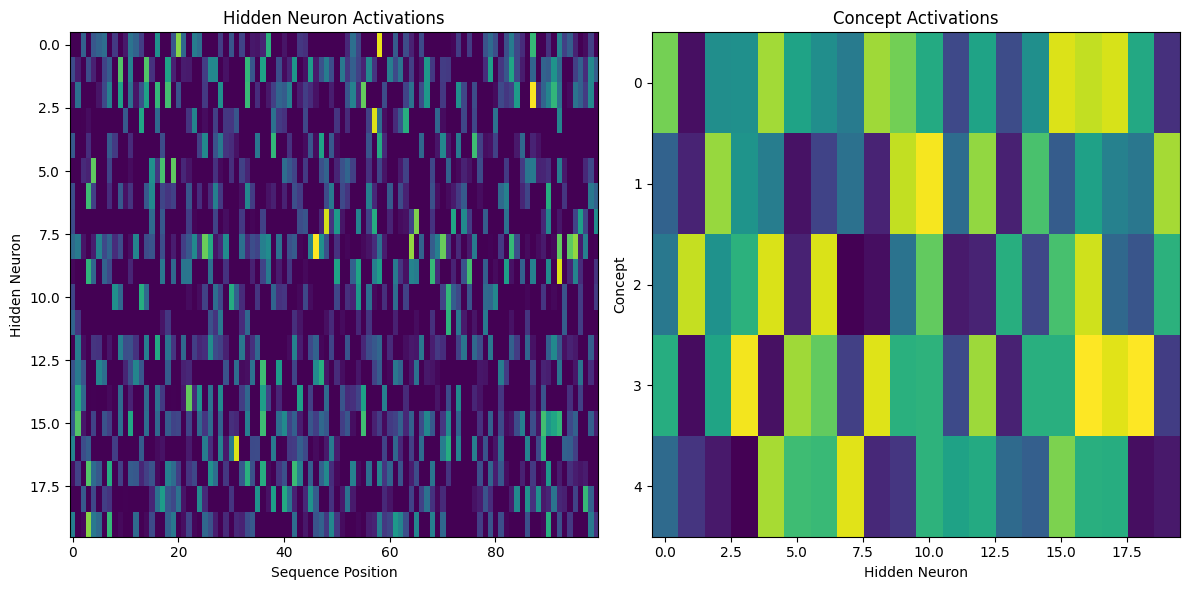
\includegraphics{language_models_files/figure-pdf/cell-3-output-1.png}

\begin{verbatim}
Correlation Matrix:
tensor([[ 1.0000,  0.2627, -0.0627,  0.0544,  0.1577, -0.2853],
        [ 0.2627,  1.0000,  0.0604, -0.0051,  0.5944,  0.3043],
        [-0.0627,  0.0604,  1.0000,  0.0394,  0.1046, -0.1701],
        [ 0.0544, -0.0051,  0.0394,  1.0000, -0.2142,  0.0359],
        [ 0.1577,  0.5944,  0.1046, -0.2142,  1.0000, -0.1420],
        [-0.2853,  0.3043, -0.1701,  0.0359, -0.1420,  1.0000]])
\end{verbatim}

\subsection{Interpretation}\label{interpretation-2}

In these visualizations, we see multiple concepts encoded in the same
set of neurons.

In the first (left) subplot, we a heatmap of activations for each hidden
neuron in the input sequence.

\begin{itemize}
\tightlist
\item
  Each row represents a single neuron in the hidden layer
\item
  Each column represents a position in the input sequence
\item
  The color intensity indicates the activation strength of each neuron
  at each position, with brighter colors showing higher activation
\end{itemize}

In the second, \emph{concept activations} visualization, we see a
heatmap showing activation patterns for different \emph{concepts} across
the hidden neurons.

\begin{itemize}
\tightlist
\item
  Rows represent different concepts
\item
  Columns represent neurons in the hidden layer
\item
  Color intensity indicates how strongly each concept is associated with
  each hidden neuron
\item
  Brighter colors indicate stronger activations
\end{itemize}

\subsection{The key idea}\label{the-key-idea}

These two visualizations overlap in hidden neuron space, so the same set
of neurons are encoding \emph{both} sequence and concept information
simultaneously. That these two aspects coexist in the same hidden layer
demonstrates superposition.

\begin{Shaded}
\begin{Highlighting}[]
\ImportTok{import}\NormalTok{ torch}
\ImportTok{import}\NormalTok{ torch.nn }\ImportTok{as}\NormalTok{ nn}
\ImportTok{import}\NormalTok{ numpy }\ImportTok{as}\NormalTok{ np}
\ImportTok{from}\NormalTok{ transformers }\ImportTok{import}\NormalTok{ DistilBertTokenizer, DistilBertModel}
\ImportTok{from}\NormalTok{ datasets }\ImportTok{import}\NormalTok{ load\_dataset}
\ImportTok{import}\NormalTok{ matplotlib.pyplot }\ImportTok{as}\NormalTok{ plt}
\ImportTok{import}\NormalTok{ seaborn }\ImportTok{as}\NormalTok{ sns}
\ImportTok{from}\NormalTok{ sklearn.decomposition }\ImportTok{import}\NormalTok{ PCA}

\CommentTok{\# Check if CUDA is available}
\NormalTok{device }\OperatorTok{=}\NormalTok{ torch.device(}\StringTok{"cuda"} \ControlFlowTok{if}\NormalTok{ torch.cuda.is\_available() }\ControlFlowTok{else} \StringTok{"cpu"}\NormalTok{)}
\BuiltInTok{print}\NormalTok{(}\SpecialStringTok{f"Using device: }\SpecialCharTok{\{}\NormalTok{device}\SpecialCharTok{\}}\SpecialStringTok{"}\NormalTok{)}

\CommentTok{\# Load pre{-}trained model and tokenizer}
\NormalTok{model\_name }\OperatorTok{=} \StringTok{"distilbert{-}base{-}uncased"}
\NormalTok{tokenizer }\OperatorTok{=}\NormalTok{ DistilBertTokenizer.from\_pretrained(model\_name)}
\NormalTok{model }\OperatorTok{=}\NormalTok{ DistilBertModel.from\_pretrained(model\_name).to(device)}

\CommentTok{\# Load a subset of the GLUE dataset (SST{-}2 for sentiment analysis)}
\NormalTok{dataset }\OperatorTok{=}\NormalTok{ load\_dataset(}\StringTok{"glue"}\NormalTok{, }\StringTok{"sst2"}\NormalTok{, split}\OperatorTok{=}\StringTok{"train[:1000]"}\NormalTok{)}

\CommentTok{\# Tokenize the dataset}
\KeywordTok{def}\NormalTok{ tokenize\_function(examples):}
    \ControlFlowTok{return}\NormalTok{ tokenizer(examples[}\StringTok{"sentence"}\NormalTok{], padding}\OperatorTok{=}\StringTok{"max\_length"}\NormalTok{, truncation}\OperatorTok{=}\VariableTok{True}\NormalTok{, max\_length}\OperatorTok{=}\DecValTok{128}\NormalTok{, return\_tensors}\OperatorTok{=}\StringTok{"pt"}\NormalTok{)}

\NormalTok{tokenized\_dataset }\OperatorTok{=}\NormalTok{ dataset.}\BuiltInTok{map}\NormalTok{(tokenize\_function, batched}\OperatorTok{=}\VariableTok{True}\NormalTok{, remove\_columns}\OperatorTok{=}\NormalTok{dataset.column\_names)}
\NormalTok{tokenized\_dataset.set\_format(}\StringTok{"torch"}\NormalTok{)}

\CommentTok{\# Define linguistic concepts (simple version)}
\NormalTok{concepts }\OperatorTok{=}\NormalTok{ \{}
    \StringTok{"positive"}\NormalTok{: [}\StringTok{"good"}\NormalTok{, }\StringTok{"great"}\NormalTok{, }\StringTok{"excellent"}\NormalTok{, }\StringTok{"wonderful"}\NormalTok{, }\StringTok{"fantastic"}\NormalTok{],}
    \StringTok{"negative"}\NormalTok{: [}\StringTok{"bad"}\NormalTok{, }\StringTok{"terrible"}\NormalTok{, }\StringTok{"awful"}\NormalTok{, }\StringTok{"horrible"}\NormalTok{, }\StringTok{"poor"}\NormalTok{],}
    \StringTok{"neutral"}\NormalTok{: [}\StringTok{"okay"}\NormalTok{, }\StringTok{"fine"}\NormalTok{, }\StringTok{"average"}\NormalTok{, }\StringTok{"mediocre"}\NormalTok{, }\StringTok{"so{-}so"}\NormalTok{]}
\NormalTok{\}}

\CommentTok{\# Function to get hidden states}
\KeywordTok{def}\NormalTok{ get\_hidden\_states(batch):}
\NormalTok{    inputs }\OperatorTok{=}\NormalTok{ \{k: v.to(device) }\ControlFlowTok{for}\NormalTok{ k, v }\KeywordTok{in}\NormalTok{ batch.items() }\ControlFlowTok{if}\NormalTok{ k }\KeywordTok{in}\NormalTok{ [}\StringTok{\textquotesingle{}input\_ids\textquotesingle{}}\NormalTok{, }\StringTok{\textquotesingle{}attention\_mask\textquotesingle{}}\NormalTok{]\}}
    \ControlFlowTok{with}\NormalTok{ torch.no\_grad():}
\NormalTok{        outputs }\OperatorTok{=}\NormalTok{ model(}\OperatorTok{**}\NormalTok{inputs)}
    \ControlFlowTok{return}\NormalTok{ outputs.last\_hidden\_state.cpu().numpy()}

\CommentTok{\# Get hidden states for the dataset}
\NormalTok{hidden\_states }\OperatorTok{=}\NormalTok{ []}
\ControlFlowTok{for}\NormalTok{ i }\KeywordTok{in} \BuiltInTok{range}\NormalTok{(}\DecValTok{0}\NormalTok{, }\BuiltInTok{len}\NormalTok{(tokenized\_dataset), }\DecValTok{32}\NormalTok{):}
\NormalTok{    batch }\OperatorTok{=}\NormalTok{ tokenized\_dataset[i:i}\OperatorTok{+}\DecValTok{32}\NormalTok{]}
\NormalTok{    hidden\_states.append(get\_hidden\_states(batch))}

\NormalTok{hidden\_states }\OperatorTok{=}\NormalTok{ np.concatenate(hidden\_states, axis}\OperatorTok{=}\DecValTok{0}\NormalTok{)}

\CommentTok{\# Calculate average hidden state for each input}
\NormalTok{avg\_hidden\_states }\OperatorTok{=}\NormalTok{ np.mean(hidden\_states, axis}\OperatorTok{=}\DecValTok{1}\NormalTok{)}

\CommentTok{\# Perform PCA}
\NormalTok{pca }\OperatorTok{=}\NormalTok{ PCA(n\_components}\OperatorTok{=}\DecValTok{2}\NormalTok{)}
\NormalTok{reduced\_states }\OperatorTok{=}\NormalTok{ pca.fit\_transform(avg\_hidden\_states)}

\CommentTok{\# Visualize the reduced hidden states}
\NormalTok{plt.figure(figsize}\OperatorTok{=}\NormalTok{(}\DecValTok{12}\NormalTok{, }\DecValTok{8}\NormalTok{))}
\NormalTok{scatter }\OperatorTok{=}\NormalTok{ plt.scatter(reduced\_states[:, }\DecValTok{0}\NormalTok{], reduced\_states[:, }\DecValTok{1}\NormalTok{], c}\OperatorTok{=}\NormalTok{dataset[}\StringTok{"label"}\NormalTok{], cmap}\OperatorTok{=}\StringTok{"coolwarm"}\NormalTok{, alpha}\OperatorTok{=}\FloatTok{0.6}\NormalTok{)}
\NormalTok{plt.colorbar(scatter)}
\NormalTok{plt.title(}\StringTok{"PCA of Average Hidden States Colored by Sentiment"}\NormalTok{)}
\NormalTok{plt.xlabel(}\StringTok{"First Principal Component"}\NormalTok{)}
\NormalTok{plt.ylabel(}\StringTok{"Second Principal Component"}\NormalTok{)}
\NormalTok{plt.show()}

\CommentTok{\# Function to get concept embeddings}
\KeywordTok{def}\NormalTok{ get\_concept\_embeddings(concepts):}
\NormalTok{    concept\_embeddings }\OperatorTok{=}\NormalTok{ \{\}}
    \ControlFlowTok{for}\NormalTok{ concept, words }\KeywordTok{in}\NormalTok{ concepts.items():}
\NormalTok{        embeddings }\OperatorTok{=}\NormalTok{ []}
        \ControlFlowTok{for}\NormalTok{ word }\KeywordTok{in}\NormalTok{ words:}
\NormalTok{            inputs }\OperatorTok{=}\NormalTok{ tokenizer(word, return\_tensors}\OperatorTok{=}\StringTok{"pt"}\NormalTok{).to(device)}
            \ControlFlowTok{with}\NormalTok{ torch.no\_grad():}
\NormalTok{                outputs }\OperatorTok{=}\NormalTok{ model(}\OperatorTok{**}\NormalTok{inputs)}
\NormalTok{            embeddings.append(outputs.last\_hidden\_state.mean(dim}\OperatorTok{=}\DecValTok{1}\NormalTok{).cpu().numpy())}
\NormalTok{        concept\_embeddings[concept] }\OperatorTok{=}\NormalTok{ np.mean(embeddings, axis}\OperatorTok{=}\DecValTok{0}\NormalTok{).flatten()}
    \ControlFlowTok{return}\NormalTok{ concept\_embeddings}

\NormalTok{concept\_embeddings }\OperatorTok{=}\NormalTok{ get\_concept\_embeddings(concepts)}

\CommentTok{\# Calculate correlation between average hidden states and concept embeddings}
\NormalTok{correlations }\OperatorTok{=}\NormalTok{ \{\}}
\ControlFlowTok{for}\NormalTok{ concept, embedding }\KeywordTok{in}\NormalTok{ concept\_embeddings.items():}
\NormalTok{    corr }\OperatorTok{=}\NormalTok{ np.mean([np.corrcoef(avg\_state, embedding)[}\DecValTok{0}\NormalTok{, }\DecValTok{1}\NormalTok{] }\ControlFlowTok{for}\NormalTok{ avg\_state }\KeywordTok{in}\NormalTok{ avg\_hidden\_states])}
\NormalTok{    correlations[concept] }\OperatorTok{=}\NormalTok{ corr}

\CommentTok{\# Visualize correlations}
\NormalTok{plt.figure(figsize}\OperatorTok{=}\NormalTok{(}\DecValTok{10}\NormalTok{, }\DecValTok{6}\NormalTok{))}
\NormalTok{sns.barplot(x}\OperatorTok{=}\BuiltInTok{list}\NormalTok{(correlations.keys()), y}\OperatorTok{=}\BuiltInTok{list}\NormalTok{(correlations.values()))}
\NormalTok{plt.title(}\StringTok{"Average Correlation between Hidden States and Concept Embeddings"}\NormalTok{)}
\NormalTok{plt.ylabel(}\StringTok{"Correlation"}\NormalTok{)}
\NormalTok{plt.show()}

\BuiltInTok{print}\NormalTok{(}\StringTok{"Correlations:"}\NormalTok{, correlations)}
\end{Highlighting}
\end{Shaded}

\begin{verbatim}
Using device: cuda
\end{verbatim}

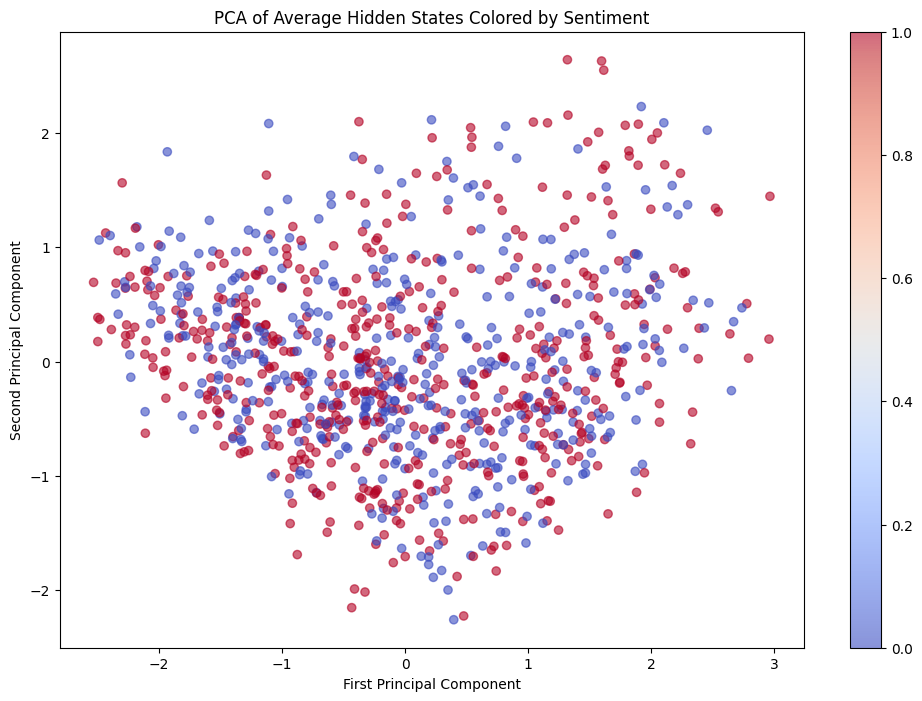
\includegraphics{language_models_files/figure-pdf/cell-4-output-2.png}

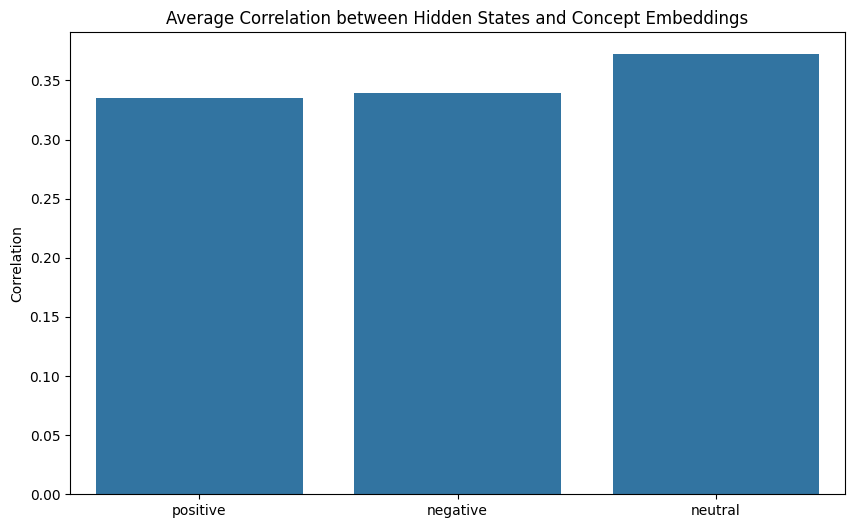
\includegraphics{language_models_files/figure-pdf/cell-4-output-3.png}

\begin{verbatim}
Correlations: {'positive': 0.33541225356469684, 'negative': 0.3389937145819827, 'neutral': 0.37208967616205857}
\end{verbatim}

\subsection{Interpretation}\label{interpretation-3}

In the PCA plot, we see clusters of points with different colors,
suggesting the model is distinguishing between different sentiments in
its hidden representations.

In the correlation bar plot, the higher values suggest hidden states are
more tightly correlated with that particular concept. The high
correlations for multiple concepts suggests the model is encoding
multiple concepts simultaneously in its hidden states.

\bookmarksetup{startatroot}

\chapter{Interpreting with Sparse
Autoencoders}\label{interpreting-with-sparse-autoencoders}

\begin{Shaded}
\begin{Highlighting}[]
\OperatorTok{!}\NormalTok{pip install torch transformers}
\end{Highlighting}
\end{Shaded}

In this notebook, we will explore one of the cutting-edge approaches to
interpreting superposition: \emph{sparse autoencoders} (SAE).

SAEs are a type of neural network used in unsupervised learning and
feature extraction. Autoencoders are generally useful for detecting
patterns that are difficult for humans to discern. SAEs have the
following characteristics:

\begin{itemize}
\tightlist
\item
  An encoder to compress data and a decoder to recontruct it
\item
  The SAE enforces sparsity in the hidden layer, activating a small
  number of neurons for a given input
\item
  This sparsity forces the network to learn more efficient and
  meaningful representations of the input data
\item
  Trained to minimize reconstruction error
\item
  Useful for feature learning, dimensionality reduction, data denoising
\end{itemize}

Let's import GPT-2 for examination and set up a simple SAE.

\begin{Shaded}
\begin{Highlighting}[]
\ImportTok{import}\NormalTok{ torch}
\ImportTok{import}\NormalTok{ torch.nn }\ImportTok{as}\NormalTok{ nn}
\ImportTok{import}\NormalTok{ torch.optim }\ImportTok{as}\NormalTok{ optim}
\ImportTok{from}\NormalTok{ transformers }\ImportTok{import}\NormalTok{ GPT2LMHeadModel, GPT2Tokenizer}
\ImportTok{import}\NormalTok{ matplotlib.pyplot }\ImportTok{as}\NormalTok{ plt}
\ImportTok{import}\NormalTok{ seaborn }\ImportTok{as}\NormalTok{ sns}

\CommentTok{\# Set up device}
\NormalTok{device }\OperatorTok{=}\NormalTok{ torch.device(}\StringTok{"cuda"} \ControlFlowTok{if}\NormalTok{ torch.cuda.is\_available() }\ControlFlowTok{else} \StringTok{"cpu"}\NormalTok{)}

\CommentTok{\# Load pre{-}trained GPT{-}2 model}
\NormalTok{model\_name }\OperatorTok{=} \StringTok{\textquotesingle{}gpt2\textquotesingle{}}
\NormalTok{tokenizer }\OperatorTok{=}\NormalTok{ GPT2Tokenizer.from\_pretrained(model\_name)}
\NormalTok{gpt2\_model }\OperatorTok{=}\NormalTok{ GPT2LMHeadModel.from\_pretrained(model\_name).to(device)}

\CommentTok{\# Define Sparse Autoencoder}
\KeywordTok{class}\NormalTok{ SparseAutoencoder(nn.Module):}
    \KeywordTok{def} \FunctionTok{\_\_init\_\_}\NormalTok{(}\VariableTok{self}\NormalTok{, input\_dim, hidden\_dim):}
        \BuiltInTok{super}\NormalTok{(SparseAutoencoder, }\VariableTok{self}\NormalTok{).}\FunctionTok{\_\_init\_\_}\NormalTok{()}
        \VariableTok{self}\NormalTok{.encoder }\OperatorTok{=}\NormalTok{ nn.Linear(input\_dim, hidden\_dim)}
        \VariableTok{self}\NormalTok{.decoder }\OperatorTok{=}\NormalTok{ nn.Linear(hidden\_dim, input\_dim)}

    \KeywordTok{def}\NormalTok{ forward(}\VariableTok{self}\NormalTok{, x):}
\NormalTok{        encoded }\OperatorTok{=}\NormalTok{ torch.relu(}\VariableTok{self}\NormalTok{.encoder(x))}
\NormalTok{        decoded }\OperatorTok{=} \VariableTok{self}\NormalTok{.decoder(encoded)}
        \ControlFlowTok{return}\NormalTok{ encoded, decoded}

\end{Highlighting}
\end{Shaded}

\begin{verbatim}
/usr/local/lib/python3.10/dist-packages/huggingface_hub/utils/_token.py:89: UserWarning: 
The secret `HF_TOKEN` does not exist in your Colab secrets.
To authenticate with the Hugging Face Hub, create a token in your settings tab (https://huggingface.co/settings/tokens), set it as secret in your Google Colab and restart your session.
You will be able to reuse this secret in all of your notebooks.
Please note that authentication is recommended but still optional to access public models or datasets.
  warnings.warn(
\end{verbatim}

\begin{verbatim}
tokenizer_config.json:   0%|          | 0.00/26.0 [00:00<?, ?B/s]
\end{verbatim}

\begin{verbatim}
vocab.json:   0%|          | 0.00/1.04M [00:00<?, ?B/s]
\end{verbatim}

\begin{verbatim}
merges.txt:   0%|          | 0.00/456k [00:00<?, ?B/s]
\end{verbatim}

\begin{verbatim}
tokenizer.json:   0%|          | 0.00/1.36M [00:00<?, ?B/s]
\end{verbatim}

\begin{verbatim}
config.json:   0%|          | 0.00/665 [00:00<?, ?B/s]
\end{verbatim}

\begin{verbatim}
model.safetensors:   0%|          | 0.00/548M [00:00<?, ?B/s]
\end{verbatim}

\begin{verbatim}
generation_config.json:   0%|          | 0.00/124 [00:00<?, ?B/s]
\end{verbatim}

The following function enables the extraction of activations from GPT-2.
The function is liberally commented to explain how to keep track of
activations.

Here's how it works: * Tokenize the text * Ensure output is a PyTorch
tensor * Return hidden states (activations) from all layers *
\texttt{output\_hidden\_states} is a tuple containing the hidden states
from all layers by \texttt{layer\_idx}, which allows us to choose which
layer's activations are of interest.

\begin{Shaded}
\begin{Highlighting}[]
\CommentTok{\# Function to get GPT{-}2 activations}
\KeywordTok{def}\NormalTok{ get\_gpt2\_activations(text, layer\_idx}\OperatorTok{={-}}\DecValTok{1}\NormalTok{):}
    \CommentTok{\# Tokenize input text; ensure output is a PyTorch (".pt") tensor}
\NormalTok{    inputs }\OperatorTok{=}\NormalTok{ tokenizer(text, return\_tensors}\OperatorTok{=}\StringTok{"pt"}\NormalTok{).to(device)}
    \CommentTok{\# Model inference, without tracking gradients. This saves memory,}
    \CommentTok{\# since we are only interested in inference, not training}
    \ControlFlowTok{with}\NormalTok{ torch.no\_grad():}
        \CommentTok{\# The output\_hidden\_states method returns the hidden states,}
        \CommentTok{\# aka activations, from all layers, not just the final output}
\NormalTok{        outputs }\OperatorTok{=}\NormalTok{ gpt2\_model(}\OperatorTok{**}\NormalTok{inputs, output\_hidden\_states}\OperatorTok{=}\VariableTok{True}\NormalTok{)}
    \CommentTok{\# outputs.hidden\_states is a tuple containing hidden states from}
    \CommentTok{\# all layers of the model. squeeze() removes extra dimensions}
    \CommentTok{\# of size 1 from the tensor.}
    \ControlFlowTok{return}\NormalTok{ outputs.hidden\_states[layer\_idx].squeeze()}
\end{Highlighting}
\end{Shaded}

\begin{Shaded}
\begin{Highlighting}[]
\KeywordTok{def}\NormalTok{ train\_sparse\_autoencoder(autoencoder, activations, num\_epochs}\OperatorTok{=}\DecValTok{500}\NormalTok{, sparsity\_weight}\OperatorTok{=}\FloatTok{0.01}\NormalTok{):}
\NormalTok{    criterion }\OperatorTok{=}\NormalTok{ nn.MSELoss()}
\NormalTok{    optimizer }\OperatorTok{=}\NormalTok{ optim.Adam(autoencoder.parameters(), lr}\OperatorTok{=}\FloatTok{0.001}\NormalTok{)}
\NormalTok{    scheduler }\OperatorTok{=}\NormalTok{ optim.lr\_scheduler.StepLR(optimizer, step\_size}\OperatorTok{=}\DecValTok{100}\NormalTok{, gamma}\OperatorTok{=}\FloatTok{0.5}\NormalTok{)}

    \ControlFlowTok{for}\NormalTok{ epoch }\KeywordTok{in} \BuiltInTok{range}\NormalTok{(num\_epochs):}
\NormalTok{        optimizer.zero\_grad()}
\NormalTok{        encoded, decoded }\OperatorTok{=}\NormalTok{ autoencoder(activations)}

\NormalTok{        recon\_loss }\OperatorTok{=}\NormalTok{ criterion(decoded, activations)}
\NormalTok{        sparsity\_loss }\OperatorTok{=}\NormalTok{ torch.mean(torch.}\BuiltInTok{abs}\NormalTok{(encoded))}
\NormalTok{        loss }\OperatorTok{=}\NormalTok{ recon\_loss }\OperatorTok{+}\NormalTok{ sparsity\_weight }\OperatorTok{*}\NormalTok{ sparsity\_loss}

\NormalTok{        loss.backward()}
\NormalTok{        optimizer.step()}
\NormalTok{        scheduler.step()}

        \ControlFlowTok{if}\NormalTok{ (epoch }\OperatorTok{+} \DecValTok{1}\NormalTok{) }\OperatorTok{\%} \DecValTok{100} \OperatorTok{==} \DecValTok{0}\NormalTok{:}
            \BuiltInTok{print}\NormalTok{(}\SpecialStringTok{f\textquotesingle{}Epoch [}\SpecialCharTok{\{}\NormalTok{epoch}\OperatorTok{+}\DecValTok{1}\SpecialCharTok{\}}\SpecialStringTok{/}\SpecialCharTok{\{}\NormalTok{num\_epochs}\SpecialCharTok{\}}\SpecialStringTok{], Loss: }\SpecialCharTok{\{}\NormalTok{loss}\SpecialCharTok{.}\NormalTok{item()}\SpecialCharTok{:.4f\}}\SpecialStringTok{\textquotesingle{}}\NormalTok{)}

    \ControlFlowTok{return}\NormalTok{ autoencoder}
\end{Highlighting}
\end{Shaded}

The following visualizations should help explain the findings of the
sparse autoencoder. One will show the strength of the activations, the
other, learned feature importance.

\begin{Shaded}
\begin{Highlighting}[]
\KeywordTok{def}\NormalTok{ visualize\_features(autoencoder, num\_features, save\_path}\OperatorTok{=}\StringTok{\textquotesingle{}learned\_features.png\textquotesingle{}}\NormalTok{):}
\NormalTok{    weights }\OperatorTok{=}\NormalTok{ autoencoder.encoder.weight.data.cpu().numpy()}
\NormalTok{    fig, axes }\OperatorTok{=}\NormalTok{ plt.subplots(}\DecValTok{4}\NormalTok{, }\DecValTok{4}\NormalTok{, figsize}\OperatorTok{=}\NormalTok{(}\DecValTok{15}\NormalTok{, }\DecValTok{15}\NormalTok{))}
    \ControlFlowTok{for}\NormalTok{ i }\KeywordTok{in} \BuiltInTok{range}\NormalTok{(num\_features):}
\NormalTok{        ax }\OperatorTok{=}\NormalTok{ axes[i }\OperatorTok{//} \DecValTok{4}\NormalTok{, i }\OperatorTok{\%} \DecValTok{4}\NormalTok{]}
\NormalTok{        sns.heatmap(weights[i].reshape(}\DecValTok{1}\NormalTok{, }\OperatorTok{{-}}\DecValTok{1}\NormalTok{), ax}\OperatorTok{=}\NormalTok{ax, cmap}\OperatorTok{=}\StringTok{\textquotesingle{}viridis\textquotesingle{}}\NormalTok{, cbar}\OperatorTok{=}\VariableTok{False}\NormalTok{)}
\NormalTok{        ax.set\_title(}\SpecialStringTok{f\textquotesingle{}Feature }\SpecialCharTok{\{}\NormalTok{i}\OperatorTok{+}\DecValTok{1}\SpecialCharTok{\}}\SpecialStringTok{\textquotesingle{}}\NormalTok{)}
\NormalTok{        ax.axis(}\StringTok{\textquotesingle{}off\textquotesingle{}}\NormalTok{)}
\NormalTok{    plt.tight\_layout()}
\NormalTok{    plt.savefig(save\_path)}
\NormalTok{    plt.close()}

\KeywordTok{def}\NormalTok{ visualize\_activation\_strengths(encoded, num\_features, save\_path}\OperatorTok{=}\StringTok{\textquotesingle{}activation\_strengths.png\textquotesingle{}}\NormalTok{):}
\NormalTok{    plt.figure(figsize}\OperatorTok{=}\NormalTok{(}\DecValTok{12}\NormalTok{, }\DecValTok{6}\NormalTok{))}
\NormalTok{    plt.bar(}\BuiltInTok{range}\NormalTok{(num\_features), encoded[:num\_features])}
\NormalTok{    plt.title(}\StringTok{\textquotesingle{}Activation Strengths of Learned Features\textquotesingle{}}\NormalTok{)}
\NormalTok{    plt.xlabel(}\StringTok{\textquotesingle{}Feature Index\textquotesingle{}}\NormalTok{)}
\NormalTok{    plt.ylabel(}\StringTok{\textquotesingle{}Activation Strength\textquotesingle{}}\NormalTok{)}
\NormalTok{    plt.xticks(}\BuiltInTok{range}\NormalTok{(}\DecValTok{0}\NormalTok{, num\_features, }\DecValTok{2}\NormalTok{))  }\CommentTok{\# Label every other feature for readability}
\NormalTok{    plt.tight\_layout()}
\NormalTok{    plt.savefig(save\_path)}
\NormalTok{    plt.close()}

\KeywordTok{def}\NormalTok{ analyze\_superposition(text, hidden\_dim}\OperatorTok{=}\DecValTok{16}\NormalTok{):}
    \CommentTok{\# Get GPT{-}2 activations}
\NormalTok{    activations }\OperatorTok{=}\NormalTok{ get\_gpt2\_activations(text).to(device)}
\NormalTok{    input\_dim }\OperatorTok{=}\NormalTok{ activations.shape[}\OperatorTok{{-}}\DecValTok{1}\NormalTok{]}

    \CommentTok{\# Initialize and train sparse autoencoder}
\NormalTok{    autoencoder }\OperatorTok{=}\NormalTok{ SparseAutoencoder(input\_dim, hidden\_dim).to(device)}
\NormalTok{    trained\_autoencoder }\OperatorTok{=}\NormalTok{ train\_sparse\_autoencoder(autoencoder, activations)}

    \CommentTok{\# Visualize learned features}
\NormalTok{    visualize\_features(trained\_autoencoder, hidden\_dim)}

    \CommentTok{\# Analyze activations}
\NormalTok{    encoded, \_ }\OperatorTok{=}\NormalTok{ trained\_autoencoder(activations)}
\NormalTok{    encoded }\OperatorTok{=}\NormalTok{ encoded.mean(dim}\OperatorTok{=}\DecValTok{0}\NormalTok{).squeeze().cpu().detach().numpy()}

    \CommentTok{\# Plot activation strengths}
\NormalTok{    visualize\_activation\_strengths(encoded, hidden\_dim)}

    \BuiltInTok{print}\NormalTok{(}\SpecialStringTok{f"Analysis complete. Check \textquotesingle{}learned\_features.png\textquotesingle{} and \textquotesingle{}activation\_strengths.png\textquotesingle{} for visualizations of }\SpecialCharTok{\{}\NormalTok{hidden\_dim}\SpecialCharTok{\}}\SpecialStringTok{ features."}\NormalTok{)}

\CommentTok{\# Run the analysis with multiple inputs}
\NormalTok{texts }\OperatorTok{=}\NormalTok{ [}
    \StringTok{"It was the best of times, it was the worst of times."}\NormalTok{,}
    \CommentTok{\# "To be or not to be, that is the question.",}
    \CommentTok{\# "In a hole in the ground there lived a hobbit.",}
    \CommentTok{\# "It was the best of times, it was the worst of times."}
\NormalTok{]}

\ControlFlowTok{for}\NormalTok{ i, text }\KeywordTok{in} \BuiltInTok{enumerate}\NormalTok{(texts):}
    \BuiltInTok{print}\NormalTok{(}\SpecialStringTok{f"}\CharTok{\textbackslash{}n}\SpecialStringTok{Analyzing text }\SpecialCharTok{\{}\NormalTok{i}\OperatorTok{+}\DecValTok{1}\SpecialCharTok{\}}\SpecialStringTok{: \textquotesingle{}}\SpecialCharTok{\{}\NormalTok{text}\SpecialCharTok{\}}\SpecialStringTok{\textquotesingle{}"}\NormalTok{)}
\NormalTok{    analyze\_superposition(text, hidden\_dim}\OperatorTok{=}\DecValTok{16}\NormalTok{)}
\end{Highlighting}
\end{Shaded}

\begin{verbatim}

Analyzing text 1: 'It was the best of times, it was the worst of times.'
Epoch [100/500], Loss: 10.9564
Epoch [200/500], Loss: 2.0957
Epoch [300/500], Loss: 1.4265
Epoch [400/500], Loss: 1.3351
Epoch [500/500], Loss: 1.3095
Analysis complete. Check 'learned_features.png' and 'activation_strengths.png' for visualizations of 16 features.
\end{verbatim}

\subsection{Learned feature
importance}\label{learned-feature-importance}

What do we mean by `features' in this example?

Models such as GPT-2 create a distributed representation of words and
concepts. Information about a single word is spread across many
dimensions of the model's internal representations, and each dimension
contributes to the representation of many different words or concepts.

GPT-2, like many transformer models, uses contextual embeddings, so the
representation of a word will change based on its context, eg the word
`bark' in sentences such as `A dog's bark' and `The bark on the tree'
will have different activations.

The sparse autoeocnder is trying to find efficient ways to encode the
patterns in the activations, rather than to isolate individual words.

\begin{Shaded}
\begin{Highlighting}[]
\ImportTok{from}\NormalTok{ IPython.display }\ImportTok{import}\NormalTok{ Image, display}

\CommentTok{\# Display the image in the notebook}
\NormalTok{image\_path }\OperatorTok{=} \StringTok{"learned\_features.png"}
\NormalTok{display(Image(filename}\OperatorTok{=}\NormalTok{image\_path))}
\end{Highlighting}
\end{Shaded}

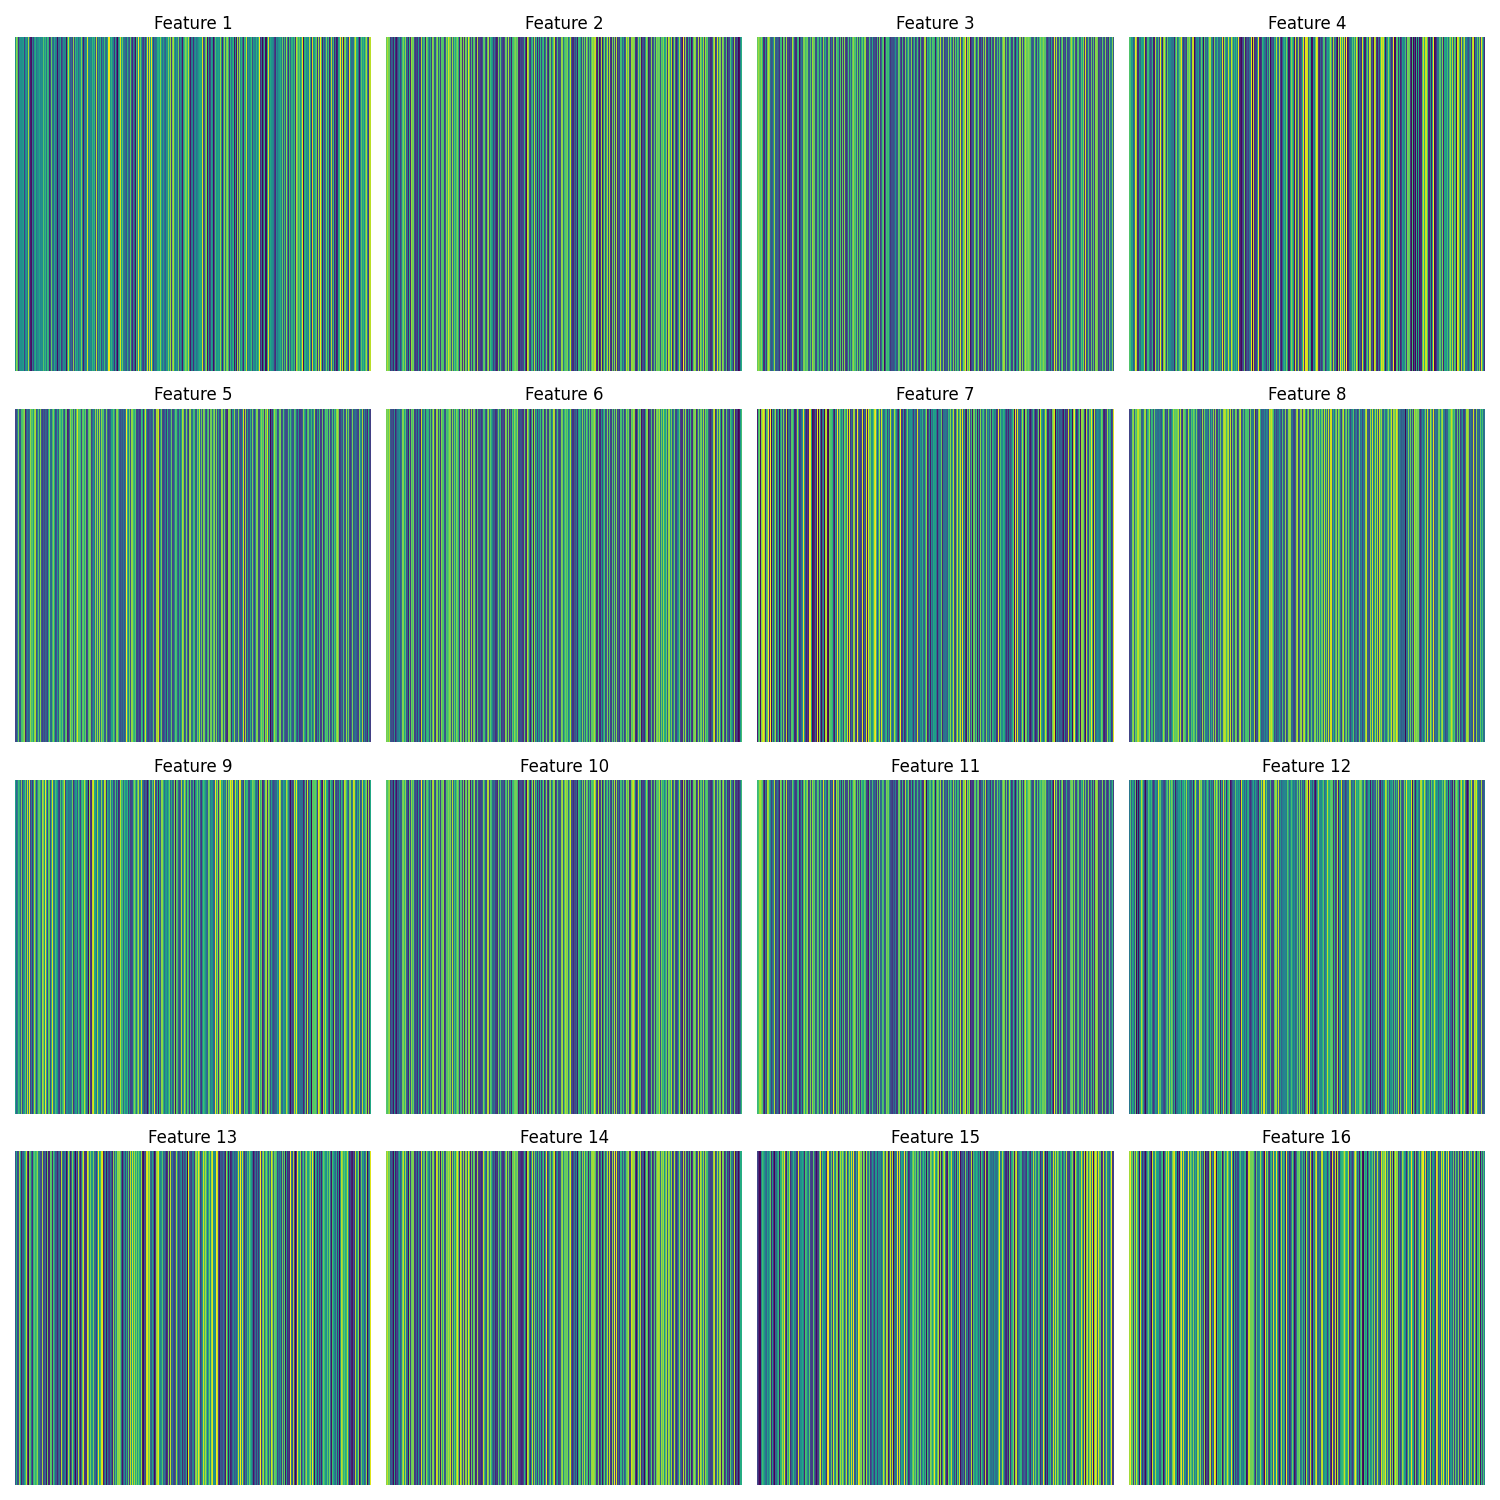
\includegraphics{sparse_autoencoders_files/figure-pdf/cell-7-output-1.png}

\subsection{Activation strengths}\label{activation-strengths}

In this visualization, high activations for some features suggest those
features are particularly relevant to representing the input sentence.
The pattern of activations across all features shows how the model is
representing the entire input.

Each bar respresents one of the features learned by the SAE, and the
height indicates how strongly the feature was activated for the input
text.

Look for sparsity: a successful sparse representation will have many
features with low activation (shorter bars), only a few will have high
activations (tall bars). The overall distribution can give clues about
how the autoencoder is representing the information.

In the GPT-2 model, the input text is distributed across all dimensions
of its activation vector, so the SAE tries to represent the same
information with fewer specific features.

\begin{Shaded}
\begin{Highlighting}[]
\ImportTok{from}\NormalTok{ IPython.display }\ImportTok{import}\NormalTok{ Image, display}

\CommentTok{\# Display the image in the notebook}
\NormalTok{image\_path }\OperatorTok{=} \StringTok{"activation\_strengths.png"}
\NormalTok{display(Image(filename}\OperatorTok{=}\NormalTok{image\_path))}
\end{Highlighting}
\end{Shaded}

\includegraphics{sparse_autoencoders_files/figure-pdf/cell-8-output-1.png}

In considering these two visualizations together, try to correlate the
strong activations in the activation strengths with feature patterns in
the heatmap.

Look for groups of features that seem to have similar patterns in the
heatmap or similar activation levels, which many indicate related
aspects of language that GPT-2 represents.

\subsection{Summary}\label{summary}

This example has shown how in the \texttt{learned\_features} heatmap how
information comprising different linguistic contexts (syntax, semantics
etc) is superposed across the same set of neurons in the original model.

In the \texttt{activation\_strengths} plot, we see how these
disentangled features are used to respresent a specific input, with
varying levels of activation indicating extracted feature relevance.

The activation of multiple features simultaneously shows how GPT-2
superposes different pieces of information in its dense representation,
which the SAE has decomposed into more interpretable units.\textbar{}

\bookmarksetup{startatroot}

\chapter{Superposition for Policy
Specialists}\label{superposition-for-policy-specialists}

In this section, we will cover what should be helpful for policy staff
to know about superposition.

\subsection{What is superposition?}\label{what-is-superposition}

Superposition in neural networks concerns how these systems efficiently
represent and process multiple concepts or features within the same set
of neurons or parameters. Unlike traditional computer programs where
every piece of information typically has a specific address in memory,
neural nets distribute this information across their entire
architecture. Information and its storage overlaps, and this helps the
network learn in greater depth from its inputs.

This feature allows neural nets to be efficieint in their use of the
computational resources they employ to help them understand input data.
The networks can understand input information with far more numerous
inputs than there are neurons to make sense of them.

\subsection{The interpretability
challenge}\label{the-interpretability-challenge}

Superposition is of interest to both research scientists and policy
experts because it presents interpretability challenges, namely the
overlapping of information makes it difficult to isolate and understand
individual concepts or how a network arrives at a prediction based on
input data. This is often refered to as the `black box' nature of AI
systems. Superposition helps robust AI systems to generalize from
training data to new inputs. However, it can also cause unexpected
behaviours when encountering scenarios significantly different to its
training data.

\subsection{Privacy}\label{privacy}

Since information is stored in a distributed fashion across the network,
privacy concerns arise since it isn't straightforward to either pinpoint
where a network keeps specific information, or how to delete it.
Information entangled with other concepts can be difficult to alter or
remove.

\subsection{Bias and fairness}\label{bias-and-fairness}

Since biased associations can be subtly encoded across many parameters
rather than in easily identifiable locations, superposition can make
identifying and mitigating bias challenging.

\subsection{Regulatory challenges}\label{regulatory-challenges}

All of the above make regulation difficult, since there is no
straightforward relationship between inputs and outputs.

\section{Avenues to improve
interpretability}\label{avenues-to-improve-interpretability}

\subsection{Visualization}\label{visualization}

We have convered some techniques in this course to apply visualizations
to detect and understand superposition.

\subsection{Proving and ablation}\label{proving-and-ablation}

Techniques to isolate specific or groups of neurons to understand
behaviour. For excellent examples, see Anthropic's work: *
\href{https://transformer-circuits.pub/2023/monosemantic-features/index.html}{Towards
Monosemanticity} * and
\href{https://transformer-circuits.pub/2023/monosemantic-features/vis/a1.html}{visualization}

\subsection{Disentanglement}\label{disentanglement}

Research focused on training networks to encourage more separated,
interpretable representations. Please see
\href{https://arxiv.org/pdf/2212.14855}{Disentangled Explanations of
Neural Network Predictions}.

\subsection{Formal theories of
representation}\label{formal-theories-of-representation}

Using mathematical frameworks to decribe how information is encoded and
processed could improve understanding.

\subsection{Explainable AI}\label{explainable-ai}

Developing tools to explain how neural nets are making decisions.

\section{Conclusion}\label{conclusion}

Superposition is a fundamental characteristic that affords neural nets
the power and complexity to make predictions and generations based on
often voluminous input data. For policy specialists, understanding this
charactersitic of AI systems helps inform the development of governance
strategies to mitigate ethical and societal impact concerns of
non-deterministic systems.

\bookmarksetup{startatroot}

\chapter{Summary}\label{summary-1}

In summary, we covered the topic of superposition, its presence in toy
models and in more sophisticated convolution neural networks and
language models. We then explored using sparse autoencoders to interpret
the features learned by the neurons in a network.

Further resources:

Coming soon

\bookmarksetup{startatroot}

\chapter*{References}\label{references}
\addcontentsline{toc}{chapter}{References}

\markboth{References}{References}

\phantomsection\label{refs}
\begin{CSLReferences}{0}{1}
\end{CSLReferences}




\end{document}
